% !TEX root =../LibroTipoETSI.tex
\chapter{Estructura de \redborderddos}\LABCHAP{CAPEstructura}
\pagestyle{esitscCD}
\epigraph{Programming is the art of telling another human what one wants the computer to do.}{Donald Knuth}

%\lettrine[lraise=0.7, lines=1, loversize=-0.25]{E}{l} 
\lettrine[lraise=-0.1, lines=2, loversize=0.25]{R}edBorder DDoS\index{RedBorder DDoS} es el nombre del producto en el 
que, mediante el análisis del tráfico en tiempo real a través del algoritmo \gls{CUSUM}, nos permite detectar ataques 
\gls{DDoS} en tiempo real. Como vimos en el \CHAP{Denegacion de Servicio}, podemos diferencias los ataques de 
\gls{DDoS} en dos grandes bloques: 
\begin{enumerate}
 \item Ataques por inundación, que buscan saturar los recursos de los que depende el servicio.
 \item Ataques semánticos. que buscan explotar una vulnerabilidad conocida.
\end{enumerate}

\redborderddos{} intenta detectar y, en la medida de lo posible, mitigar el primer tipo de ataque, mediante el 
algoritmo \gls{CUSUM} visto en el \CHAP{Algoritmo CUSUM}. Sin embargo, para manejar y ser capaz de detectar un ataque 
\gls{DDoS} por inundación, destinado a agotar los recursos de una máquina, es necesario disponer de muchos recusos y 
usar algoritmos eficientes, a fin de que el recurso agotado no sea el elemento detector del \gls{DDoS}.

Por ello, se busca aprovechar al máximo la estructura multiprocesador de los sensores de los que disponemos. El 
principal cuello de botella en este tipo de sistema son los elementos de comunicación entre los distintos núcleos y 
procesos, por lo que se buscará reducir al mínimo dicho lastre.

A lo largo de este capítulo se presenta la estructura que sigue \redborderddos{} desde el punto de vista del arquitecto 
de software y programador. Tras describir las nociones de programación necesarias y algunas particularidades de los 
algoritmos computacionales en \SEC{NocionesPrevias}. A continuación, se describirá el proyecto desde una perspectiva de 
``caja negra'', esto es, qué necesita como entrada y salida de datos para funcionar, en la \SEC{Vista Externa}. En este 
caso, \redborderddos{} funciona usando un puerto SPAN del que recibe una copia de todo el tráfico dirigido hacia el 
activo a defender.

Por último, y usando la información de los anteriores apartados, analizamos cómo funciona el programa desde un punto de 
vista interno en la sección \SEC{EstructuraInterna}, separando el mismo en varios componentes: repartidor del tráfico, 
contadores del tráfico, aglutinador de los contadores y, por último decisor. De esta forma, entendemos cómo funciona el 
programa en su conjunto, y qué tipo de ataques podemos esperar obtener de él, y en qué formato se nos presentarán, 

\section{Nociones previas}\LABSEC{NocionesPrevias}

%TODO por qué basado en C

A lo largo de este capítulo se describirá la estructura de \redborderddos. \redborderddos{} está basado en el lenguaje 
de programación C, y usa alguna característica avanzada que no todos los usuarios de C tienen por qué conocer antes de 
leer este capítulo.

Por tanto, describiremos en esta sección las técnicas usadas, a fin de que podamos hacer referencia a ellas al 
describir el funcionamiento del programa sin necesidad de mezclar detalles de bajo y alto nivel.

\subsection{Comparación de números en coma flotante}\index{Número en coma flotante}
Salvar un número decimal en la memoria de un ordenador tiene una condición importante: La memoria del ordenador es 
finita. Los números, por el contrario, son infinitos. Es más, entre dos números distinguibles cualesquiera, hay 
infinitos números reales intermedios.

Así, pues, si destinamos por ejemplo $4$ bits de memoria para guardar un número, para una misma base sólo podremos 
guardar $2^{4}$ números distintos. Si, por ejemplo, queremos guardar los números posibles entre $0$ y $1$, la 
asignación número $\rightarrow$ representación binaria quedaría como en la \TAB{RepresentacionBinariaEjemplo4bits}.

\begin{table}
\begin{tabular}{cl}
 Representación & Número \\\hline
  \texttt{0000} & 0.000000 \\
  \texttt{0001} & 0.066667 \\
  \texttt{0010} & 0.133333 \\
  \texttt{0011} & 0.200000 \\
  \texttt{0100} & 0.266667 \\
  \texttt{0101} & 0.333333 \\
  \texttt{0110} & 0.400000 \\
  \texttt{0111} & 0.466667 \\
  \texttt{1000} & 0.533333 \\
  \texttt{1001} & 0.600000 \\
  \texttt{1010} & 0.666667 \\
  \texttt{1011} & 0.733333 \\
  \texttt{1100} & 0.800000 \\
  \texttt{1101} & 0.866667 \\
  \texttt{1110} & 0.933333 \\
  \texttt{1111} & 1.000000
 \end{tabular}
 \caption{Representación posible de flotantes equidistantes desde el 0 hasta el 1 usando cuatro bits.}
 \LABTAB{RepresentacionBinariaEjemplo4bits}
\end{table}

Si, con esta representación, computamos $1/4+1/4-1/2$, el ordenador tendría que aproximarlo a 
$\mathtt{0b0100}+\mathtt{0b0100}-\mathtt{0b0111} \rightarrow 0.266667+0.266667-0.466667$, las representaciones más 
próximas de las que disponemos. Entonces, el resultado de la operación binaria sería $\mathtt{0b0001} \rightarrow 
0.066667$, y no $0$, como se esperaría en un sistema numérico real.

Pese a que en el proyecto se trabaja con números en punto flotante IEE754 dobles, capaces de almacenar $2^64$ números 
distintos, no estamos exentos de este tipo de fallos. Para evitarlos, la comparación entre números no debe ser 
realizada con el operador \texttt{==}, sino que en su lugar se compararán dejando lugar a un margen de error, como se 
ve en Algoritmo \ALG{ComparacionFlotante}.

\begin{algorithm}
 \KwData{Dos números $n_1$,$n_2$ en formato \texttt{double IEEE754}, y un epsilon $e$}
 \KwResult{Comparación de los mismos: 0 si son iguales, $>0$ si $n_1>n_2$ y $<0$ en otro caso}
 \eIf{$abs\left(n_1-n_2\right)< e$}{
   devolver 0\;
 }{
   devolver $n_1-n_2$\;
 }
 \caption{Algoritmo de comparación de números en punto flotante}
 \LABALG{ComparacionFlotante}
\end{algorithm}

\subsection{Estructuras de datos básicas}\index{Estructura de datos}
Para almacenar el funcionamiento de cada flujo de tráfico, y ser capaz de compararlo con el supuesto funcionamiento 
normal de la red, es necesario contar con unos sistemas de almacenamiento rápidos y eficientes. Si se pierde demasiado 
tiempo en el manejo de la memoria, \redborderddos{} no será capaz de leer y modelar el tráfico a una velocidad 
correcta, y a la larga no será capaz de detectar nada.

A lo largo de esta subsección describiremos las estructuras de almacenamiento de datos usadas en el programa. Una vez 
que conozcamos el funcionamiento de estas, será más fácil ver el sistema como un todo, y abstraer correctamente cada 
una de sus partes.

\subsubsection{Vector de memoria}\index{Vector}\LABSSSEC{VectorMemoria}
Un vector consiste en una o más celdas de memoria situadas de una forma contigua. Esto es, si cada elemento del vector 
ocupa $L$ bytes, y el vector comienza en la dirección de memoria $M$, podemos acceder al tercer elemento del vector en 
la dirección $M+3L$.

El vector tiene un tamaño fijo conocido en el momento de su creación, y, a lo largo de este trabajo, no variará. Hemos 
de tener precaución al acceder a las distintas posiciones del vector: si hemos reservado memoria para $K$ elementos, y 
accedemos al elemento número $J>=K$\footnote{En C, las posiciones del vector empiezan en 0. Si accedemos al elemento 
$K$, ya estamos accediendo a memoria fuera del vector}, esa zona de memoria no está dentro del vector, y no se puede 
saber qué habrá.

\subsubsection{Listas enlazadas}\index{Lista Enlazada}\LABSSSEC{ListaEnlazada}
Si, tras haber definido un tamaño de vector, queremos añadir nuevos elementos, deberíamos redimensionar el espacio 
reservado del vector en memoria. Esta es una operación costosa, ya que puede no existir espacio contiguo al final o 
principio del vector, y necesitar buscar un espacio contiguo más grande. Tras encontrarlo, se necesitará copiar todos 
los elementos del vector, y pueden ser muchos.

Aún peor, ¿qué ocurre cuando queremos insertar un elemento en mitad del vector? Es necesario mover todos los elementos 
desde la posición requerida hasta el final del vector una unidad, y después insertar ese último elemento, lo que 
resulta inadmisible.

% TODO describir NULL en el glosario?
Para solucionar este problema, podemos usar una lista tipo enlazada. En ella, cada elemento tiene un puntero que apunta 
al siguiente elemento, mientras que el último elemento de la lista siempre apuntará a NULL. Por lo tanto, insertar o 
eliminar un elemento en mitad de la lista sólo requeriría localizar el elemento anterior, y modificar dos puntero. Como 
caso especial está el insertado de elementos a la cabeza de la lista, que sólo requiere modificar dos punteros.

Podemos ver en la \FIG{EstructuraLinkedList} la estructura que tendría.

\begin{figure}[htbp]
\centering
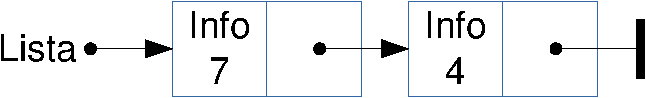
\includegraphics[width=0.5\textwidth]{CapituloEstructura/Figuras/EstructuraListaEnlazada-crop}
\caption{Estructura de una lista enlazada}
\LABFIG{EstructuraLinkedList} %Esto es una forma propia de los autores de gestionar las etiquetas y referencias
\end{figure}
%

Sin embargo, el acceso aleatorio a un elemento de la lista enlazada es algo más costoso, ya que para acceder la 
posición $N$ es necesario iterar por todos los $N-1$ elementos. Existen otras variantes, que incluyen usar un puntero 
al anterior y posterior nodo, listas circulares, listas con puntero a la cabeza y a cola, etc. Pero por el momento, nos 
basta con esta visión de las listas enlazadas.

%TODO explicar listas doblemente enlazadas, y la lista tommy.

\subsubsection{Pilas}\index{Pila}
Una pila es una estructura de datos con sólo dos operaciones: añadir elementos a la pila (operación \emph{push}) y 
extraer el último elemento de la pila (operación \emph{pop}). Si insertamos un elemento $E$, insertamos tras él $N$ 
elementos, será necesario extraer (\emph{pop}) los $N$ elementos antes de volver a acceder al elemento $E$. Es, por 
tanto, una cola \gls{LIFO}.

Podemos simular una pila con un vector de memoria, si llevamos la cuenta de los elementos que hemos insertado con una 
variable \emph{cuenta} con valor inicial a cero, podemos hacer \emph{push} salvando en dicha posición e incrementando 
esa variable, y \emph{pop} decrementandola y devolviendo la posición.

\subsubsection{Tabla HASH}\index{Tabla HASH}
Resumiendo los apartados \SSSEC{VectorMemoria} y \SSSEC{ListaEnlazada}:
\begin{itemize}
 \item Es muy rápido acceder a una posición dada de un vector, pero la inserción de elementos es potencialmente muy 
lenta. Además, mientras el vector no está lleno, desperdicias memoria
 \item El acceso aleatorio a un elemento de una lista enlazada es lento. Sin embargo, la inserción de elementos en 
cualquier punto es rápida, especialmente al principio, y no se desperdicia memoria.
\end{itemize}

La tabla HASH pretende aunar lo mejor de ambas estructuras. Una tabla HASH es un mapa asociativo, en el que cada 
\emph{valor} $V$ tiene asociada una \emph{clave} $K$ por la que puede ser buscado, y dicha clave determina una posición 
en un vector de memoria.

Internamente, el vector de memoria tiene $S$ posiciones, donde $S$ es una potencia de 2.Cada posición es una lista de 
elementos del mismo tipo que el valor que queremos almacenar.

\begin{figure}[hbtp]
\centering
%\hfill
\subfloat[Diagrama de Actividad de Inserción]%
   {\LABFIG{InsertarTablaHash}%
   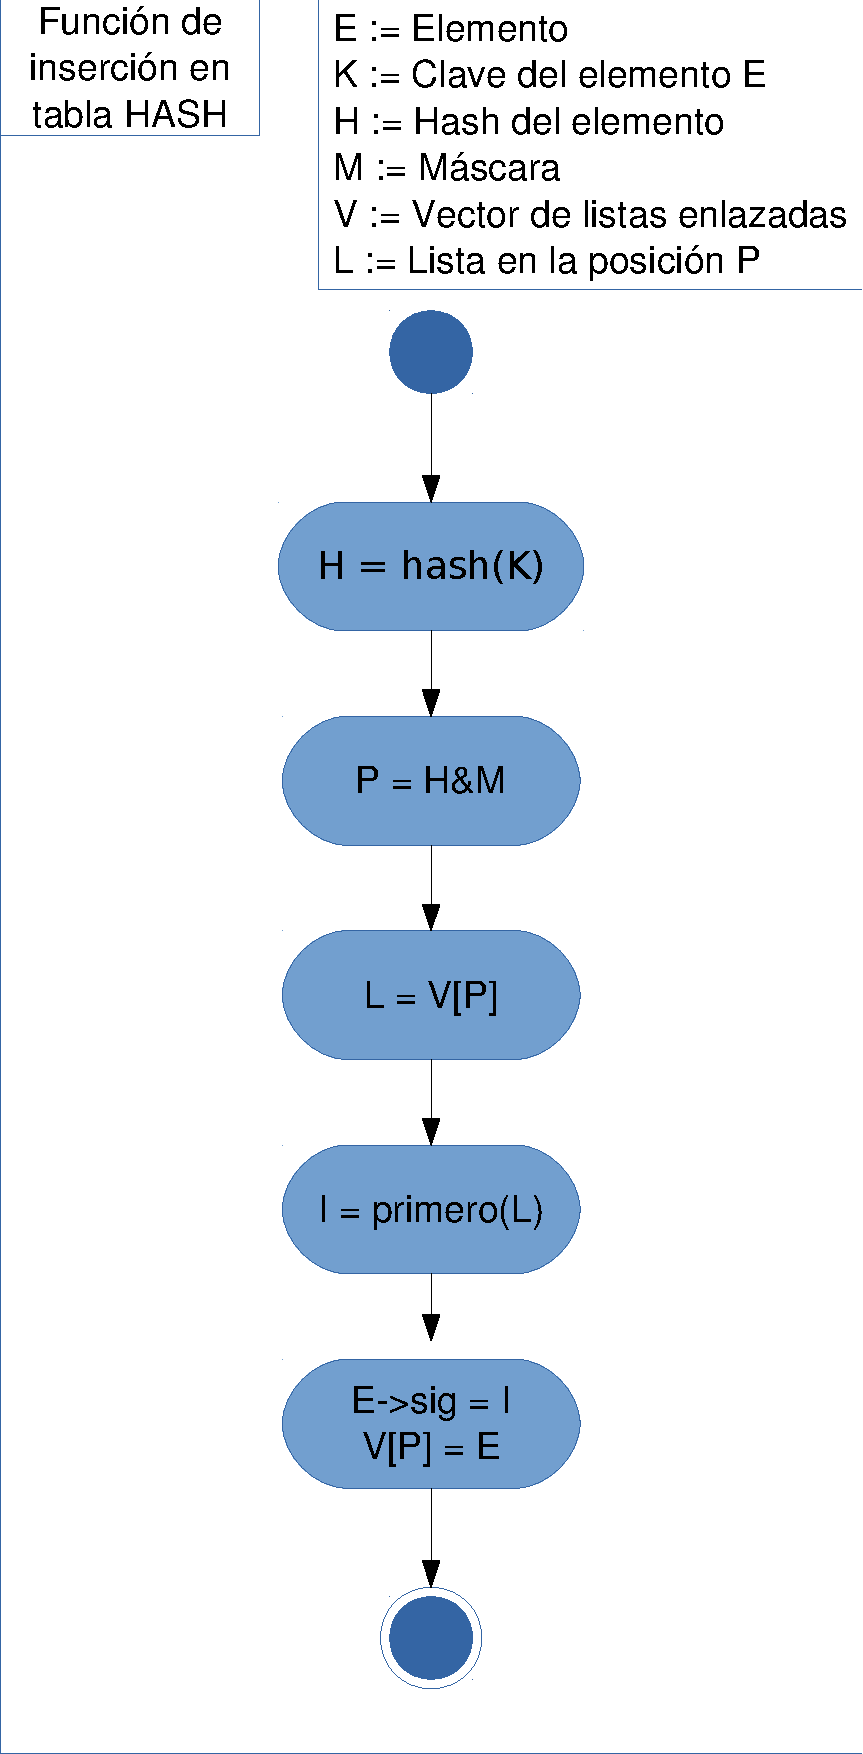
\includegraphics[width=0.48\textwidth]{CapituloEstructura/Figuras/ActividadFuncionInsertarTablaHash-crop}}%
\hfill
\subfloat[Diagrama de actividad de Búsqueda]%
 {\LABFIG{BuscarTablaHash}%
 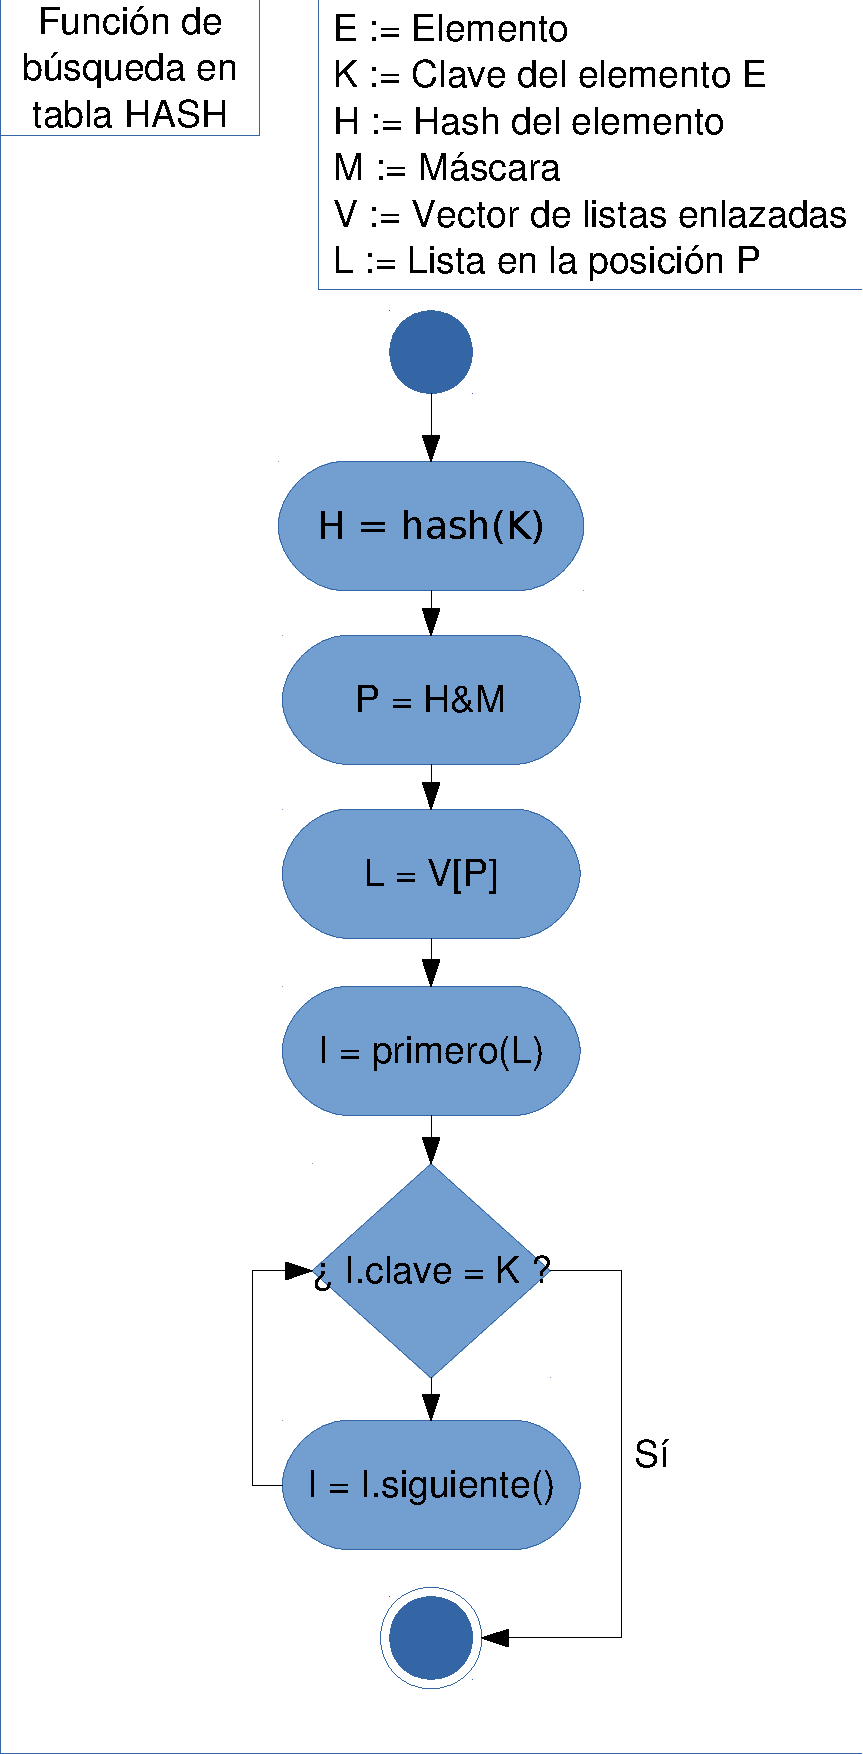
\includegraphics[width=0.48\textwidth]{CapituloEstructura/Figuras/ActividadFuncionBuscarTablaHash-crop}}%
%
\caption{Diagrama de Actividad de las operaciones a realizar sobre una tabla HASH}
\end{figure}
%

A la hora de almacenar un elemento $E_0$ con clave $K_0$, a la clave se le aplica una máscara que asegure un número 
inferior a $S$: Por ejemplo, si $S$ es $2^8$, la máscara debe ser $M=0xff$, de forma que la operación \emph{AND} bit a 
bit de siempre $P_0=K_0\&S<2^8$. El elemento $E_0$ es entonces insertado en la lista que ocupa la posición $P_0$ del 
vector de memoria. El diagrama de actividad de esta función se puede ver en \FIG{InsertarTablaHash}.

Por su parte, a la hora de recuperar el elemento, volvemos a aplicar la máscara a la clave, $P_0=K_0\&M$, y buscamos en 
la lista enlazada que ocupa la posición $P_0$ del vector. Esta vez, sí deberemos comparar los elementos con la clave 
$K$, ya que en ella existen todos los elementos insertados cuyas claves $K$ cumplan $K\&M=P_0$. Podemos ver su diagrama 
de actividad en \FIG{BuscarTablaHash}.

Para conseguir la mínima probabilidad de colisión, se le aplica a las diferentes claves una función HASH\index{Función 
HASH}, esto es una, función que ante la misma entrada de siempre la misma salida, pero que pequeñas diferencias de los 
valores de la entrada provoca grandes diferencias en los valores de salida. Como nota, es probable que una función HASH 
produzca colisiones, esto es, diferentes entradas producen la misma salida.

En el mismo sentido, es importante encontrar una buena relación entre el tamaño de la tabla hash y el número de 
elementos que queremos insertar. Siempre será más rápido que una lista puramente enlazada, pero cuantos menos elementos 
ocupen la misma posición de memoria, mejor.

%TODO reservar una sección "pruebas realizadas"

Por ejemplo, supongamos que queremos almacenar unos contadores, cuyo flujo está asociado a la \gls{IP} \emph{10.0.1.1}, 
en una tabla hash de longitud $S=2^8$. Tras aplicarle nuestra función HASH, vemos que 
$\text{hash}(\text{10.0.0.1})=476$. Buscamos en la tabla HASH la lista enlazada de la posición 
$476\&0xff=220$, y la añadimos a la cola. Ver \FIG{EstadoTablaHashInsercion} para visualizar gráficamente qué ocurre 
con la tabla HASH.

\begin{figure}[hbtp]
\centering
\subfloat[Estado antes de la inserción]%
   {\begin{minipage}[t]{0.47\textwidth}\vspace{0pt}
    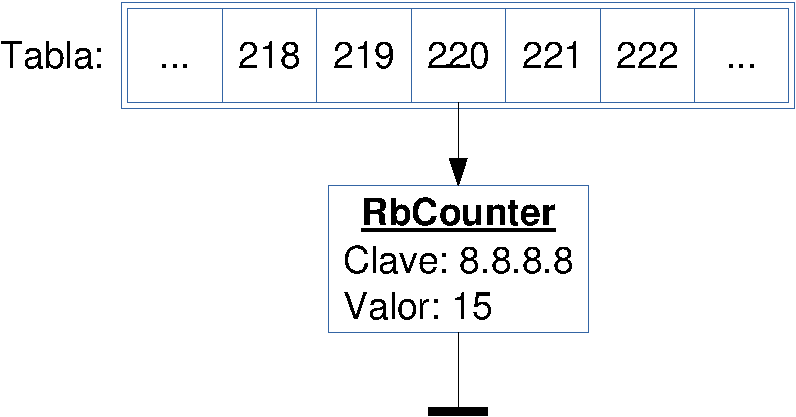
\includegraphics[width=\textwidth]{CapituloEstructura/Figuras/TablaHashAntesInsercion-crop}%
    \end{minipage}}
\hfill
\subfloat[Estado después de la inserción]%
 {\begin{minipage}[t]{0.47\textwidth}\vspace{0pt}
 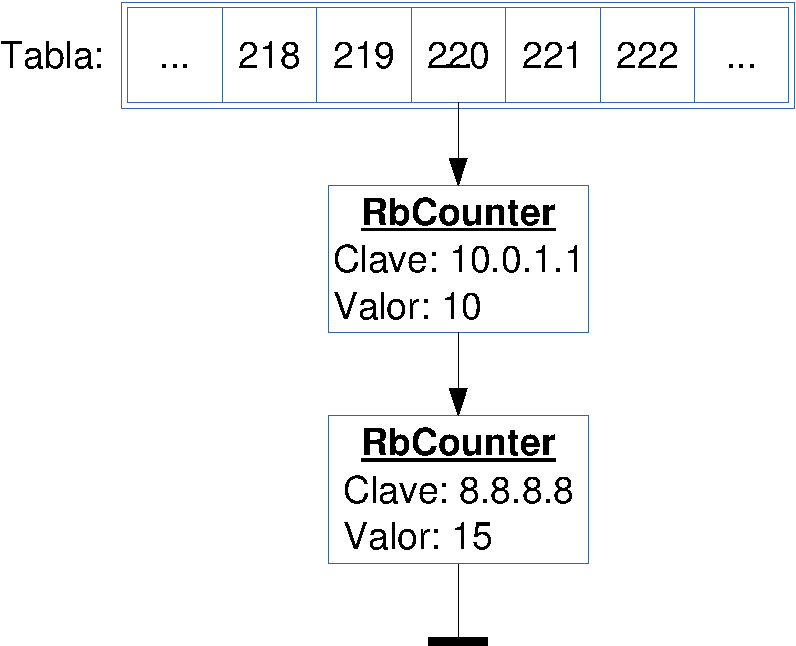
\includegraphics[width=\textwidth]{CapituloEstructura/Figuras/TablaHashDespuesInsercion-crop}%
  \end{minipage}}
%
\caption{Inserción de un elemento en la tabla HASH}
\LABFIG{EstadoTablaHashInsercion}
\end{figure}

\subsection{Programación multihilo}\LABSSEC{ProgramacionMultihilo}
Un hilo de un proceso\index{Hilo}, también llamado proceso ligero\index{Proceso Ligero}, es una forma que tienen las 
aplicaciones de ejecutar código de manera concurrente. 

Al crear un hilo, se crea una nueva entrada en el planificador\index{Planificador} del \gls{SO}, y ésta instancia se 
ejecutará con la misma prioridad que otros procesos. Tendrá su propio contador de programa\footnote{Indicador del punto 
de ejecución actual.}, su propia pila de llamada a funciones y su propio estado de CPU, lo que permite que el hilo 
llamante y el llamado se ejecuten por separado.

Sin embargo, los distintos hilos de un proceso comparten el espacio de direcciones y ficheros abiertos. Esto es útil 
para compartir memoria entre ellos, pero genera la necesidad de un mecanismo de sincronización.

Por ejemplo, supongamos una función que realiza las siguientes acciones sobre un entero de valor 0:
\begin{enumerate}
 \item Copia un entero a un registro\label{item:EjemploHilosGetInt}.
 \item Incrementa ese entero.
 \item Vuelve a guardar ese entero en su ubicación original, ya incrementado.
\end{enumerate}

Esta función se está llamando concurrentemente\index{Concurrencia} desde dos hilos distintos. Se debería esperar que, 
tras la ejecución de los dos hilos, el entero valga 2.

Sin embargo, si hilamos mas fino, descubrimos un problema. Pongamos el caso de que, en el momento de terminar la 
instrucción \ref{item:EjemploHilosGetInt}, el planificador decide que es hora de pasar el control al hilo dos. 
Éste lee la variable (de valor 0), la incrementa, y guarda un 1. Ahora, cuando el control vuelve al hilo 1, este 
simplemente tiene en su registro un 0, lo incrementará a 1, y guardará un 1. Y no podemos saber cuando el planificador 
decidirá cambiar el hilo en ejecución, por lo que este problema se puede reproducir de manera aleatoria.

Es necesaria una \emph{Variable Cerrojo}\index{Variable Cerrojo}\index{Mutex}. Una variable especial que sólo puede ser 
modificada por un proceso al mismo tiempo en todo el sistema y, por tanto, proteja la \emph{sección 
crítica}\index{Sección Crítica}, esto es, aquella susceptible de ser indeterminada si el procesador cambia de hilo de 
ejecución en el momento que está siendo ejecutada.

Por tanto, la función pasaría a ser:
\begin{enumerate}
 \item Cerramos la variable cerrojo
 \item Copia un entero a un registro
 \item Incrementa ese entero.
 \item Vuelve a guardar ese entero en su ubicación original, ya incrementado.
 \item Abrimos la variable cerrojo
\end{enumerate}

De esta forma, ambos hilos de ejecución saben cuando otro proceso está modificando la \emph{región crítica}.

No obstante, esto tiene una desventaja: el hilo que espera a que la variable cerrojo sea abierta no puede hacer otra 
cosa que no sea esperar. Por tanto, una mala elección de secciones críticas hará el programa lento.

\subsection{Alineamiento de datos en memoria}
El alineamiento\index{Alineamiento de Datos}\index{Alineamiento de memoria} de los datos se refiere a obligar a que un 
tipo de dato específico ocupe una cierta cantidad de octetos en memoria, y comience en una dirección de memoria 
determinada.

Esto significa que, por ejemplo, si tenemos una estructura que ocupa $40$ bytes en memoria, el compilador obligará a 
que esta ocupe $64$ bytes, rellenando la parte sobrante con ``basura''. A priori, esto parece un derroche de memoria, 
pero tiene varias ventajas si entendemos cómo funcionan los procesadores y el acceso a memoria a bajo nivel.

\subsubsection{Inconvenientes de no alinear con un procesador}\LABSSSEC{NoAlinearUnProcesador}
Un procesador es capaz de trabajar, de forma directa, con bloques alineados de memoria o palabras. Por ejemplo, 
establecer a cero una estructura de $40$ bytes llevaría dos instrucciones: Establecer a $0$ los primeros $32$ bytes, y 
establecer a $0$ los $8$ bytes restantes. El resto de bytes no se pueden tocar, ya que pueden pertenecer a cualquier 
otra cosa. Por ejemplo, si esas estructuras fuesen un vector en memoria, pertenecerían a la estructura que ocupase el 
siguiente índice.

Sin embargo, un procesador sí puede establecer a $0$ una página de $64$ bytes de memoria con una sola instrucción, ya 
que sabemos que los bytes restantes serán basura.

Por otra parte, suponiendo que, en el anterior vector la posición $i$ esté alineada, es seguro que el elemento $i+1$ no 
estará alineado. Sin embargo, el procesador sólo es capaz de leer\footnote{En realidad, de llevar a su memoria caché}, 
de una vez, páginas alineadas. Eso obligará al elemento que ocupa dos páginas realizar dos accesos distintos a la 
caché: la primera, para leer la primera parte del elemento, y la segunda para leer el resto. Por último, necesitará una 
última instrucción para unir las anteriores lecturas. Podemos ver una descripción gráfica en 
\FIG{AccesoMemoriaNoAlineada}.

Sin embargo, si el elemento sólo ocupa una página de memoria, o un múltiplo de ésta, estamos seguros de poder traernos 
ese elemento en sólo una iteración, evitando así operaciones innecesarias. Se puede ver este modo de funcionar en la 
figura \FIG{AccesoMemoriaAlineada} \cite{intelAlignment}.

\begin{figure}[hbtp]
\centering
%\hfill
\subfloat[Acceso del procesador a memoria no alineada]%
   {\LABFIG{AccesoMemoriaNoAlineada}%
   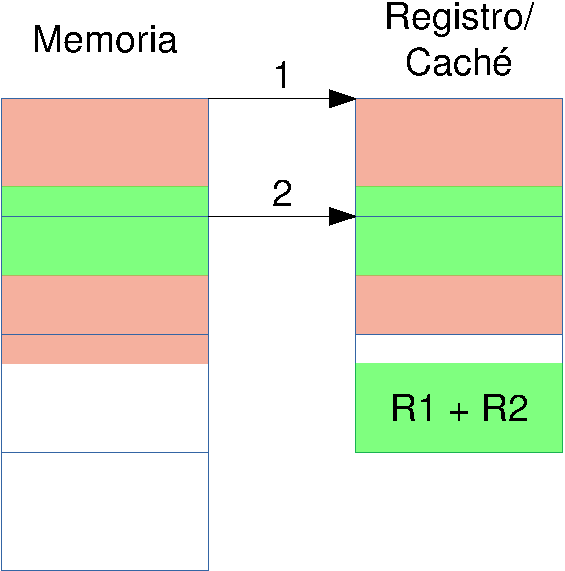
\includegraphics[width=0.45\textwidth]{CapituloEstructura/Figuras/AccesoMemoriaNoAlineada-crop}}
\hfill
\subfloat[Acceso del procesador a memoria alineada]%
   {\LABFIG{AccesoMemoriaAlineada}%
   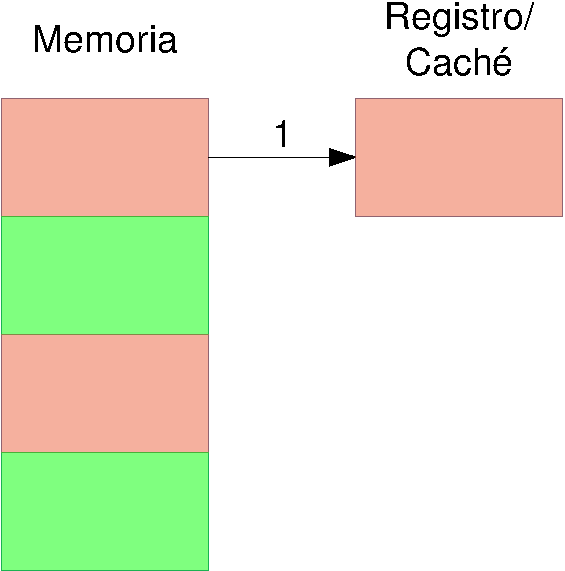
\includegraphics[width=0.45\textwidth]{CapituloEstructura/Figuras/AccesoMemoriaAlineada-crop}}
%
\caption{Diferencia entre el acceso a bloques de memorias alineados y no alineados}
\end{figure}
%

\subsubsection{Inconvenientes de no alinear con más de un procesador}
Por motivos de sincronización, todos los procesadores deben notificar qué memoria están modificando. De no hacerlo, dos 
modificaciones muy rápidas podrían solaparse y el estado de la memoria sería indeterminado.

Siguiendo con el mismo ejemplo que en el \SSSEC{NoAlinearUnProcesador}, es posible que el elemento $i$ del vector lo 
esté procesando un procesador, y, al mismo tiempo, el elemento $i+1$ esté situado en la caché de otro. Si esto sucede, 
y las modificaciones son muy frecuentes, se perderá un montón de tiempo en sincronización. Es lo que se conoce como 
\emph{cache miss}\index{Cache Miss}.

Sin embargo, si cada elemento ocupa una sóla página de caché, sin solaparse con las siguientes, garantizamos que la 
comunicación entre núcleos sea innecesaria \cite{intelAlignmentSMP}.

\subsubsection{Alineamiento de memoria con gcc}
Para evitarlo, se suele añadir una palabra clave a la declaración de las estructuras. En el caso del compilador gcc, 
que será el usado en el proyecto, dicha palabra es \texttt{\_\_aligned}. Por ejemplo, si queremos que una estructura 
con tres enteros esté alineada en memoria, se declarará como en \lstlistingname{}\ref{code:structAlignment} 
\cite{gccTypeAttributes}.

\begin{lstlisting}[language=C++,caption={Alineamiento de una estructura de datos}, 
breaklines=true, label=code:structAlignment,numbers=left,float=htbp]
 struct S { int f[3]; } __attribute__ ((aligned));
\end{lstlisting}

\subsection{Señales en linux. La señal SIGALRM.}\LABSSEC{SIGALRM}\index{SIGALRM}\index{Señal Linux}
Un mecanismo de comunicación entre procesos o \gls{IPC} es el envío de señales. Por ejemplo, cuando un programa intenta 
escribir en un área de memoria restringida, el \gls{SO} le envía una señal \gls{SIGSEGV}, y el proceso puede actuar en 
consecuencia.

Cuando un proceso la recibe, pueden ocurrir tres cosas según la señal. Por defecto, o es ignorada, o abortará el 
programa. No obstante, también es posible escribir código para manejar algunas señales.

En este caso, cuando el proceso decida crear un manejador para una señal\index{Manejador de señal Linux} concreta, y 
reciba dicha señal, será interrumpido y será como si en ese momento hubiese llamado al manejador. Cuando el manejador 
termine, el programa seguirá su ejecución normal. Si el programa estaba en un \texttt{sleep}, este será interrumpido, y 
el programa no dormirá los segundos restantes.

Por ejemplo, si pulsamos \texttt{Ctrol-Z} en un programa, este detendrá su ejecución y podremos o bien enviarlo a 
segundo plano con el comando \texttt{bg} o reanudar su ejecución con \texttt{fg}. Esto es notificado al programa con 
una señal \gls{SIGTSTP}, y es posible manejarla.

Por ejemplo, el \lstlistingname{} \ref{code:dumbSignalStopHandling} muestra un ejemplo de manejo de esta señal. Sin 
embargo si varias señales llegan muy rápido, comenzaremos a manejar una señal mientras aún estábamos manejando la 
anterior, por lo que tenemos el mismo problema que en \SSEC{ProgramacionMultihilo}. Para colmo, no podemos solucionarlo 
con una variable cerrojo: \gls{pthreads}\index{Librería phtread} establece que el resultado de bloquear una señal 
bloqueada por tu mismo hilo de ejecución es indeterminado. Y esto podría pasar si el manejador de la señal salta en la 
región crítica.

\begin{lstlisting}[language=C++,caption={Manejo ingenuo de la señal \gls{SIGTSTP}}, 
breaklines=true, label=code:dumbSignalStopHandling,numbers=left,float=htbp]
#include <signal.h>
#include <stdio.h>

#define N 10
static int i = 0;
static int salir = 0;

static void manejador(int signo){
    if(i++<N)
        printf("¡No quiero parar!\n");
    else
        salir = 1;
}

int main(void) {
     signal(SIGTSTP, manejador);
     while (!salir)
         sleep(1);
     return 0;
}
\end{lstlisting}

Así pues, la solución pasa por reducir al mínimo la responsabilidad del manejador de la señal: Este sólo establecerá un 
indicador global de que la señal ha sido recibida, y el manejador real estará en un hilo y, por tanto, en un entorno 
controlado. Vemos un ejemplo de este modo de proceder en \lstlistingname{} \ref{code:SignalStopHandling}

\begin{lstlisting}[language=C++,caption={Manejo de la señal \gls{SIGTSTP}}, 
breaklines=true, label=code:SignalStopHandling,numbers=left,float=htbp]
#include <signal.h>
#include <stdio.h>

#define N 10
static int sig = 0;

static void manejador(int signo){
    sig = 1;
}

int main(void) {
     int i = 0;
     signal(SIGTSTP, manejador);
     while (i<N){
        sleep(1);
        if(sig){
            printf("¡No quiero salir!\n");
            ++i;
            sig = 0;
        }
    }
    return 0;
}
\end{lstlisting}

Por último, una señal interesante, y que usaremos en el proyecto, es la señal \gls{SIGALRM}\index{Señal 
\texttt{SIGALRM}}. Mediante la función \texttt{alarm(int s)}\index{Función \texttt{alarm}}, se le notifica al \gls{SO} 
de que se desea recibir una señal \gls{SIGALRM} pasados \texttt{s} segundos. Por tanto, se podría usar para realizar 
tareas periódicas. Por ejemplo, el \lstlistingname{} \ref{code:AlarmSignal} imprimirá la fecha actual\footnote{En 
formato \emph{UNIX time}\index{UNIX time}, esto es, segundos transcurridos desde el 1 de Enero de 1970} y un mensaje 
indicativo de que se está realizando alguna tarea.

\begin{lstlisting}[language=C++,caption={Ejemplo de uso de \gls{SIGALRM}}, 
breaklines=true, label=code:AlarmSignal,numbers=left,float=htbp]
#include <signal.h>
#include <stdio.h>
#include <time.h>   // time()
#include <unistd.h> // alarm()

static int alarma = 0;

static void manejador(int signo){
    alarma = 1;
    alarm(1); // Programamos la siguiente alarma
}

int main(void) {
     signal(SIGALRM, manejador);
     alarm(1);
     while (1){
        sleep(1);
        if(alarma){
            printf("[%d] Estoy haciendo cosas...\n",time(NULL));
            // Sleep(100)
            alarma = 0;
        }
    }
    return 0;
}
\end{lstlisting}

Sin embargo, este programa vuelve a ignorar la concurrencia. ¿Qué ocurre si el programa tarda mas de la cuenta en 
ejecutarse? Si des-comentamos el \texttt{sleep(100)} entre el \texttt{printf(...)} y el \texttt{alarma = 0}, vemos que 
el programa imprime el mensaje cada dos segundos, en lugar de cada segundo. Esto es debido a que se ha lanzado la 
alarma mientras se estaba ejecutando el trabajo (el \texttt{sleep}), y nada ha cambiado tras ello (ya que sólo hemos 
establecido \texttt{alarma} a 1, pero ya estaba a 1). Debido a ello, es posible que el trabajo no se esté ejecutando 
con la periodicidad que nosotros creemos.

Para solucionarlo, se hace necesario otra variable que indique que una señal ha llegado mas tarde de la cuenta. En 
\lstlistingname{} \ref{code:AlarmSignalAcumulados}. 

Por último, no se debe confiar en hacer de \texttt{acumulados} un contador, ya que la alarma podría saltar en cualquier 
momento entre el \texttt{if(acumulados)} y el \texttt{acumulados=0}. Es necesario confiar en otros sistemas, como 
almacenar la marca de tiempo en la que el proceso fue lanzado.

\begin{lstlisting}[language=C++,caption={Ejemplo de uso de \gls{SIGALRM} con detección de pérdidas}, breaklines=true, 
label=code:AlarmSignalAcumulados,numbers=left,float=htbp]
#include <signal.h>
#include <stdio.h>
#include <time.h>   // time()
#include <unistd.h> // alarm()

static int alarma = 0;
static int acumulados = 0;

static void manejador(int signo){
    if(alarma)
        acumulados = 1; // Aún no ha acabado el anterior trabajo
    alarma = 1;
    alarm(1); // Programamos la siguiente alarma
}

int main(void) {
     signal(SIGALRM, manejador);
     alarm(1);
     while (1){
        sleep(1);
        if(alarma){
            if(acumulados){
                printf("[%d] Nos hemos saltado alguna iteración.",time(NULL));
                printf(" Se actuará en consecuencia.\n");
                acumulados = 0;
            }
            printf("[%d] Estoy haciendo cosas...\n",time(NULL));
            sleep(100);
            alarma = 0; // Todo vuelve a la normalidad
        }
    }
    return 0;
}
\end{lstlisting}

\section{Vista externa}\LABSEC{Vista Externa}
\subsection{Situación física de \redborderddos}
Desde el punto de vista de la arquitectura de red, \redborderddos{} debe colocarse en dos puertos SPAN\index{Puerto 
SPAN} del conmutador que llegue al activo protegido, tal y como muestra la \FIG{diagramaArquitectura}. Cada uno de los 
puertos SPAN clonará los paquetes dirigidos hacia el activo a proteger, y los paquetes desde el activo a proteger 
respectivamente, y los enviará hacia \redborderddos.

\begin{figure}[htbp]
\centering
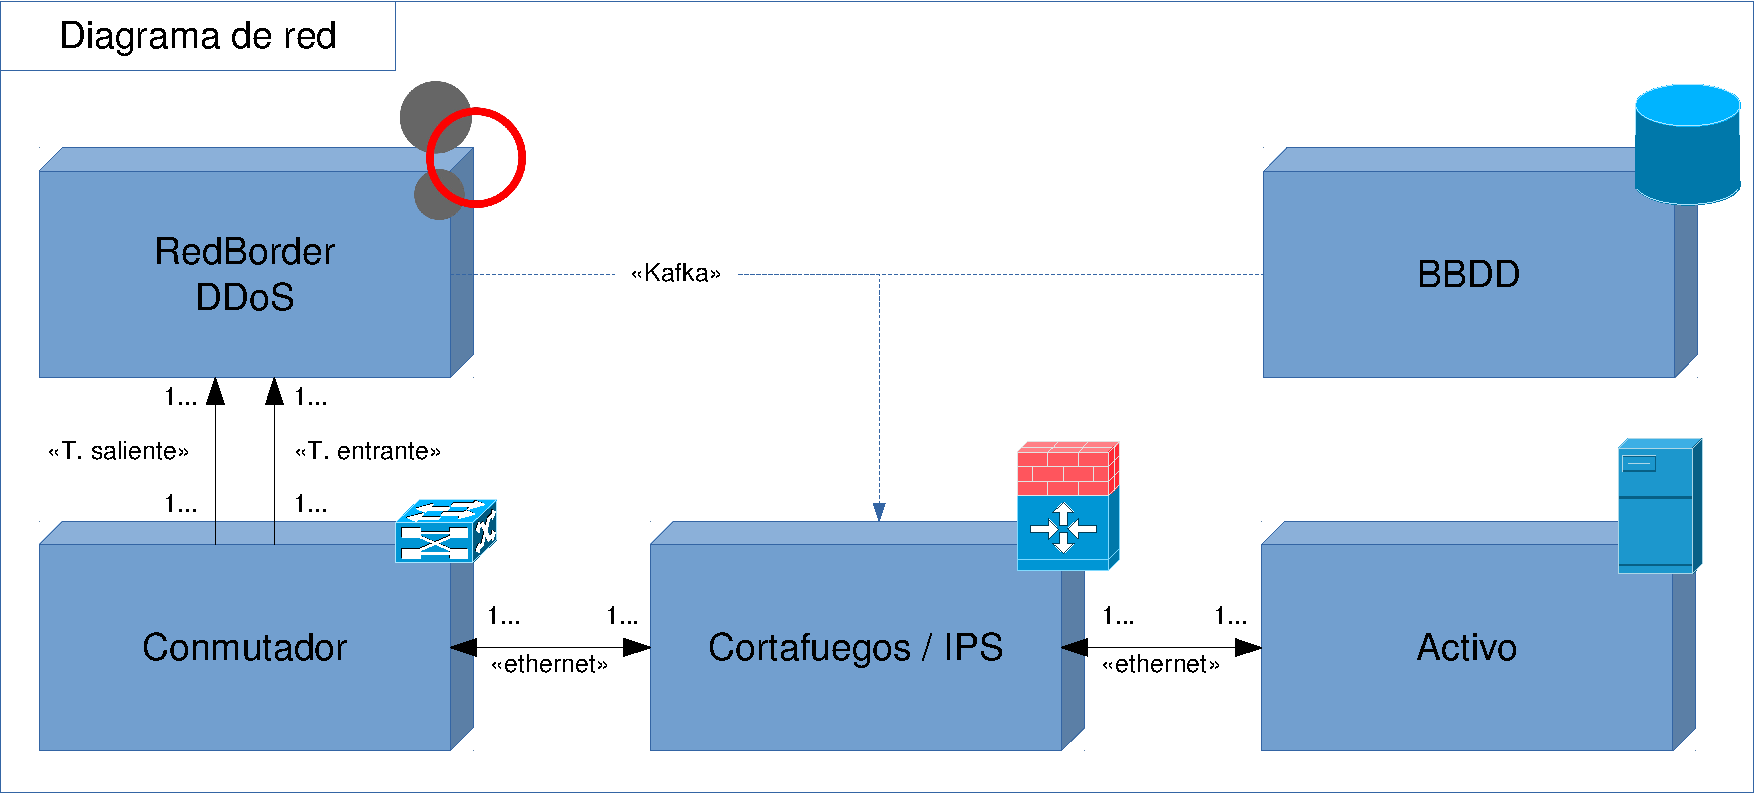
\includegraphics[width=\textwidth]{CapituloEstructura/Figuras/DiagramaArquitectura-crop}
\caption{Diagrama de Arquitectura de \redborderddos}
\LABFIG{diagramaArquitectura} %Esto es una forma propia de los autores de gestionar las etiquetas y referencias
\end{figure}
%

Tras el conmutador, se debería colocar un cortafuegos o \gls{IPS}, que se usa para:
\begin{enumerate}
 \item Detener el tráfico detectado como atacante por \redborderddos.
 \item Detener ataques semánticos o usuarios no autorizados.
\end{enumerate}

\redborderddos{} puede funcionar sin el cortafuegos\index{Cortafuegos}. No obstante, en ese caso sólo detectaremos los 
ataques, en lugar de detenerlos efectivamente.

Es necesario que \redborderddos{} se coloque delante del elemento que corta el tráfico. De otra forma, sería imposible 
para el sistema conocer cuándo ha cesado el ataque, y cuándo podemos dejar el Modo Alerta.

Podemos ver en el diagrama que podríamos multiplicar los puertos de SPAN. Esto es, si tenemos demasiado tráfico y no es 
posible enviarlo todo por un sólo puerto, podemos dedicar a \redborderddos{} dos puertos de entrada y dos de salida. 
Incluso, podríamos dedicar dos o más puertos de entrada, y sólo uno de tráfico saliente, si el tráfico que tenemos es 
altamente asimétrico. Cualquier combinación es posible, siempre y cuando tengamos al menos un puerto destinado a cada 
dirección. De esta forma, \redborderddos{} es completamente escalable desde un punto de vista de admisión de datos.

\subsection{Registro y alerta del ataque. El protocolo Apache Kafka}
% TODO ver formato del registro: Disco duro y por kafka
Cuando un ataque se produce, \redborderddos{} es capaz de registrarlo en un fichero de texto plano del disco duro y 
enviarlo por la plataforma Apache Kafka\index{Apache Kafka}.

Apache Kafka es un protocolo de transferencia de mensajes que sigue un modelo de intercambiador o 
\emph{broker}\index{Kafka Broker}. Está diseñado para ser distribuido y extensible \cite{ApacheKafka}, por lo que si 
encontramos mucha carga de trabajo, es posible aumentar, de manera horizontal\footnote{Esto es, doblar el número de 
nodos debe doblar, aproximadamente, el rendimiento obtenido.}, la capacidad de procesamiento, siempre y cuando 
dispongamos de máquinas (reales o virtuales) que sirvan de nodos Kafka.

Así, \redborderddos{} es un productor Kafka\index{Productor Kafka}, que envía el registro de ataques a una cola de 
mensajes a un \emph{broker}, que los almacenará y entregará al consumidor\index{Consumidor Kafka} que los solicite.

Muchos sistemas de procesamiento de eventos usan Apache Kafka como base para su funcionamiento. Por ejemplo, es posible 
enriquecer los eventos con Apache Storm\index{Apache Storm} \cite{ApacheStorm}, o bien almacenarlos en una base de 
datos orientada a documentos como MongoDB\index{MongoDB} \cite{MongoDB}, mucho más rápida a la hora de almacenar este 
tipo de eventos que las bases de datos relacionales usadas tradicionalmente.

\subsection{Mitigación del ataque}
Para mitigar el ataque, es necesario que exista un cortafuegos\index{Cortafuegos} o un \gls{IPS}\index{Intrusion 
Prevention System} que bloquee el tráfico dirigido al activo a proteger. Una vez que éste existe, es necesaria una vía 
de comunicación con el mismo. Actualmente, \redborderddos{} simplemente alerta de los ataques, por lo que sería 
necesario que el \gls{IPS} o algún sistema intermedio leyese de la cola Kakfa y modificase su comportamiento en base a 
dicha lectura.

\section{Estructura interna}\LABSEC{EstructuraInterna}
Internamente, \redborderddos{} intenta aprovechar al máximo la potencia de procesamiento del sensor, haciendo todas las 
tareas posibles de una manera concurrente.

Para ello, separaremos en distintos núcleos\footnote{Entendidos como núcleos de procesadores físicos.} del sensor los 
distintos bloques funcionales en los que se divide el proyecto, representados en la figura \FIG{diagramaActividad}. A 
saber:

\begin{description}
 \item [Clúster] La función del clúster es agrupar los paquetes entrantes y salientes de las distintas 
interfaces, indicar el sentido del mismo, y dirigirlos a las distintas colas que los sub-contadores leen.
 \item [Sub-contadores] Los sub-contadores agrupan todos los paquetes entrantes por flujos según IP externa, y 
contabilizan los distintos valores necesarios para ejecutar el algoritmo \gls{CUSUM} por cada flujo.
 \item [Contador Maestro y Decisor] El contador maestro, cada periodo de tiempo definido, recoge los contadores de cada 
sub-contador y aplica el algoritmo \gls{CUSUM} sobre ellos. Por su parte, el decisor se encarga de comparar dichos 
valores con los valores límite, identificando la IP como atacante si encontramos que una de ellas los sobrepasa.
\end{description}

\begin{figure}[htbp]
\centering
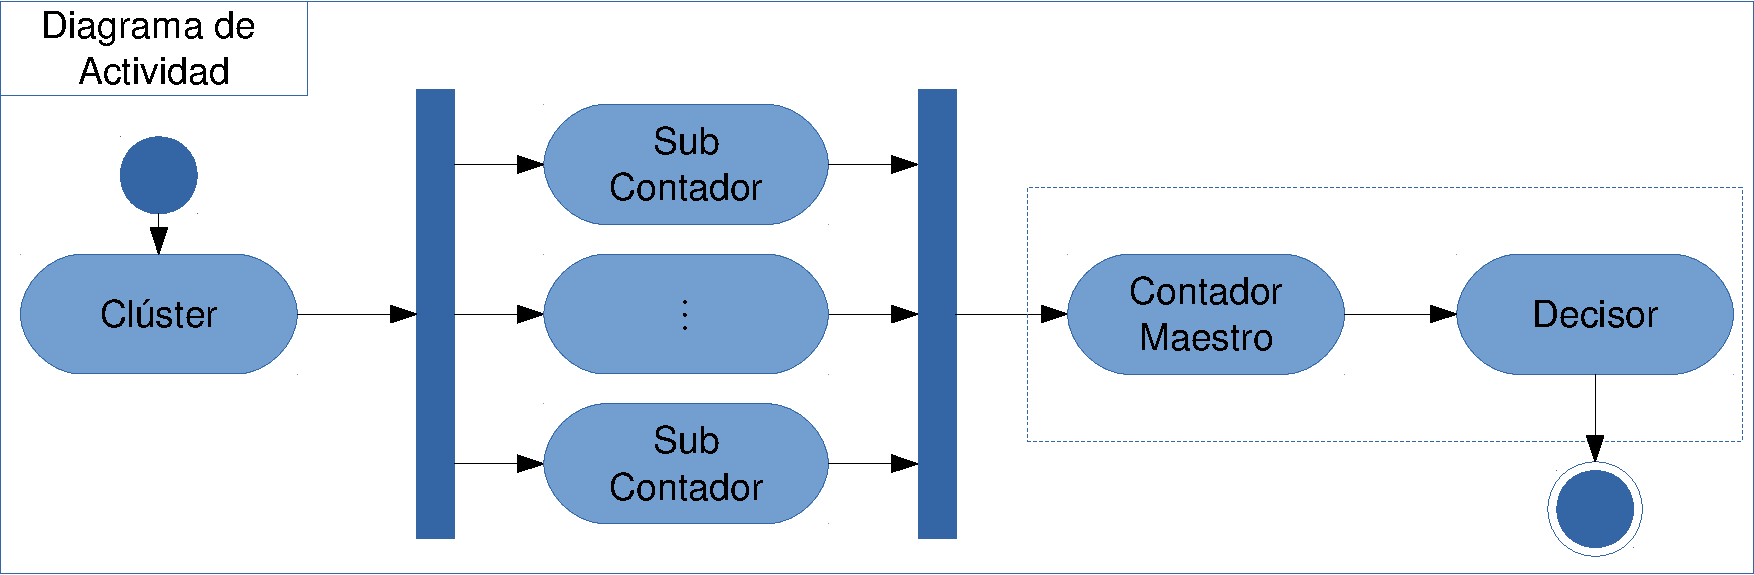
\includegraphics[width=\textwidth]{CapituloEstructura/Figuras/DiagramaFlow-crop}
\caption{Diagrama de Actividad de \redborderddos}
\LABFIG{diagramaActividad}
\end{figure}
%

\subsection{Clúster}\index{PF\_RING Cluster}\LABSSEC{EstructuraCluster}
Un clúster \acrshort{PFRING}\footnote{En \CHAP{PFRING} se detallará qué es \acrshort{PFRING}. Por el 
momento, es sólo el nombre concreto de este tipo de clúster.} es capaz de dividir todo el troncal de tráfico recogido 
por una o varias interfaces en una o más colas, de forma que cada cola vea sólo una porción del tráfico, de una manera 
coherente.

\begin{figure}[htbp]
\centering
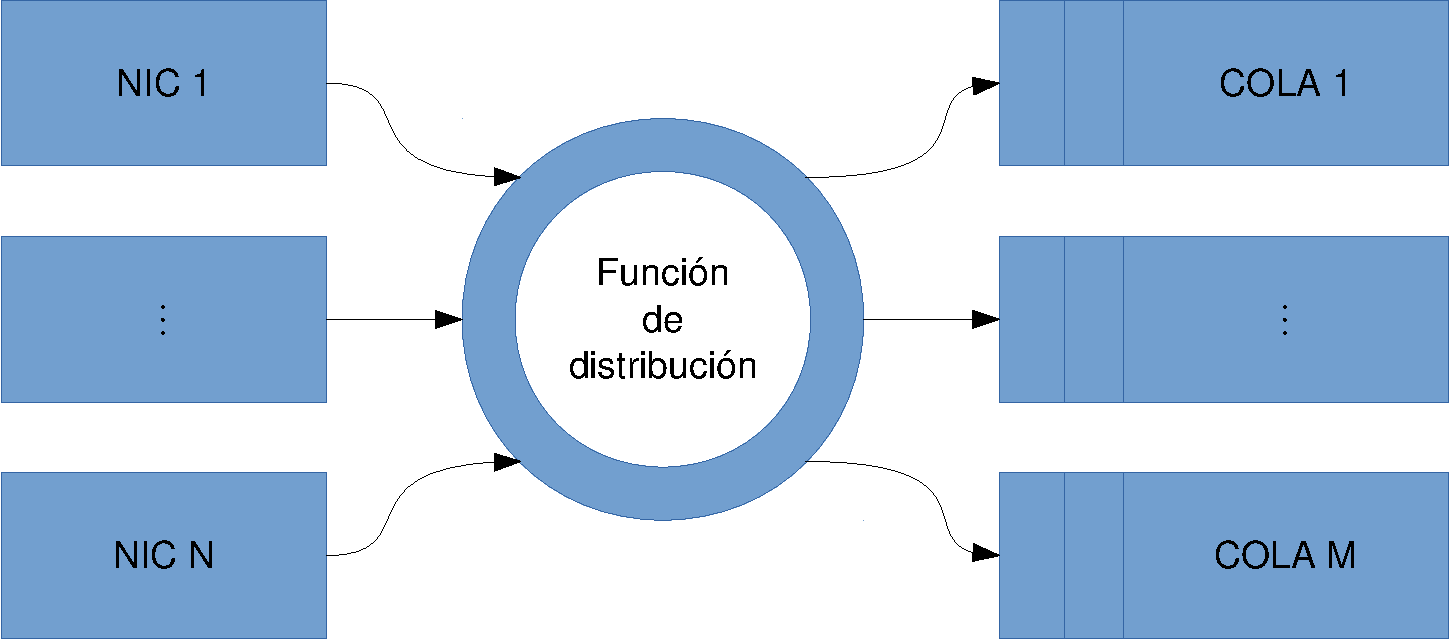
\includegraphics[width=0.75\textwidth]{CapituloEstructura/Figuras/Cluster-crop}
\caption{Funcionamiento del clúster}
\LABFIG{Cluster}
\end{figure}
%

La función de distribución es completamente definible: Podríamos haber decidido enviar los paquetes en 
\emph{round-robbin}, esto es, uno a cada cola cada vez.

La forma de reenvío que hemos elegido es por tupla (\emph{IP origen},\emph{IP destino}) de manera simétrica, esto es, 
la petición y la respuesta de un mismo flujo siempre irá dirigido a la misma cola. De esta forma, como se verá más 
adelante, cada hilo contador (ver \SSEC{subcontadores}) sólo ve una parte del flujo coherente, y el contador maestro, a 
la hora de agrupar todos los flujos, tendrá que hacer muchas menos operaciones, ya que nunca se tendrán que sumar dos 
registros.

Por otra parte, la función de distribución marcará el paquete como entrante o saliente, según haya llegado por una 
interfaz definida como tal.

Al multiplexar de esta forma las colas, conseguimos reducir el número de inter-bloqueos, ya que en 
logar de tener un modelo en el que muchos hilos atacan una misma cola, cada hilo sólo mirará su propia cola,, y en cada 
cola sólo podrán actuar dos bloqueantes (el cluster y el hilo).

De esta forma, conseguimos transparencia y escalabilidad en el número de interfaces de entrada de datos, e 
incrementamos el rendimiento a la hora de agrupar los paquetes.

Se puede ver el gráficamente el algoritmo seguido por la función de distribución en el diagrama de actividad de la 
\FIG{ActividadDistribFunc}.

\begin{figure}[htbp]
\centering
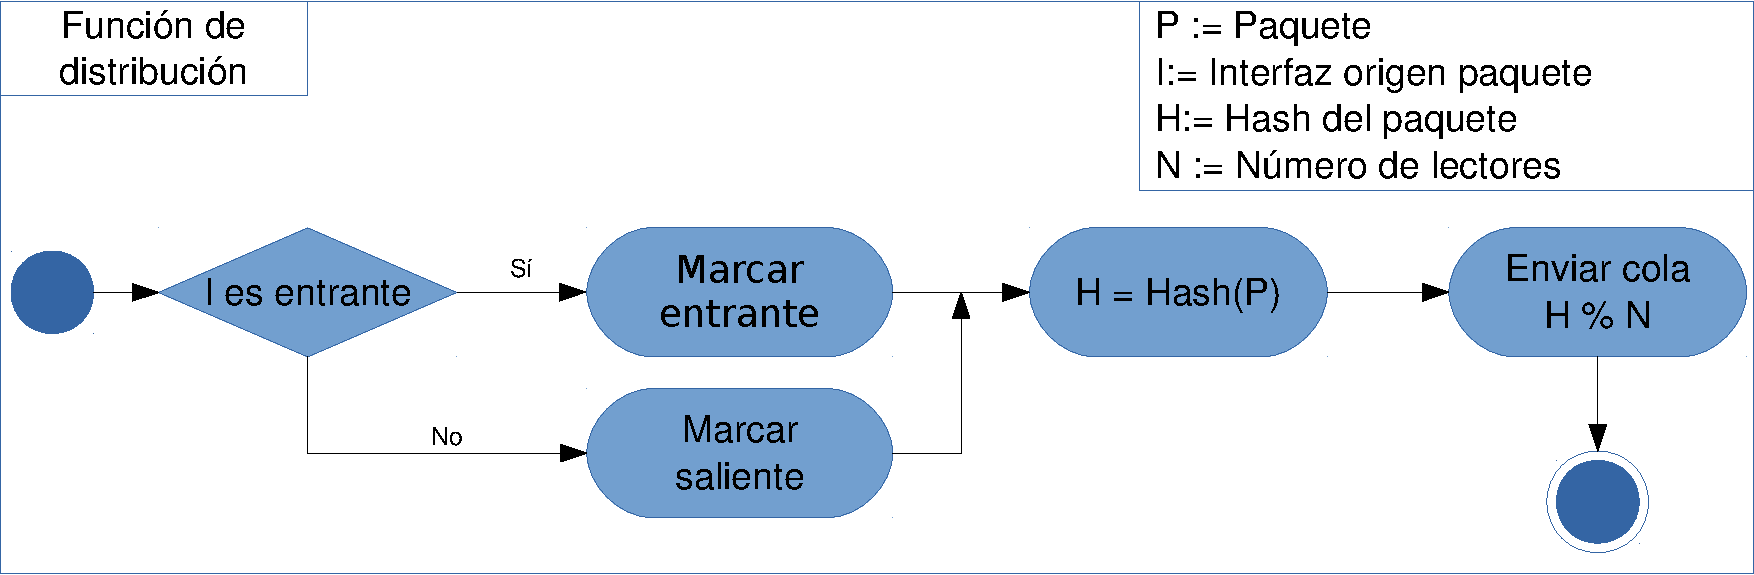
\includegraphics[width=\textwidth]{CapituloEstructura/Figuras/ActividadFuncionDistribucionCluster-crop}
\caption{Función de distribución}
\LABFIG{ActividadDistribFunc}
\end{figure}
%

\subsection{Subcontadores}\index{Subcontador}\LABSSEC{subcontadores}
\subsubsection{Estructura contador}
Con el fin de almacenar las características del tráfico descritas en \SSEC{Parametros de interés}, se prepara una 
estructura de datos en la que se irán contando los paquetes y octetos de cada tipo. Dicha estructura de datos puede 
verse en \lstlistingname{} \ref{code:RbCounter}. Por comodidad, dicha estructura también será llamada, a lo largo del 
proyecto, simplemente \texttt{RbCounter}.

\begin{lstlisting}[language=C++,caption={Estructura de contadores por flujo}, breaklines=true, 
label=code:RbCounter,numbers=left,float=htbp]
typedef uint32_t counter_t;

typedef struct rb_counters_s{
    rb_addr_t external_address; ///< External IP address

    counter_t tcp_pkts;     ///< number tcp packets in the flow
    counter_t udp_pkts;     ///< number udp packets in the flow
    counter_t icmp_pkts;    ///< number icmp packets in the flow
    counter_t total_pkts;   ///< total number packets in the flow

    counter_t tcp_bytes;    ///< tcp bytes in the flow
    counter_t udp_bytes;    ///< udp bytes in the flow
    counter_t icmp_bytes;   ///< icmp bytes in the flow
    counter_t total_bytes;  ///< total bytes in the flow

    counter_t input_pkts;   ///< Input packets in the flow;
    counter_t output_pkts;  ///< Output packets in the flow;
    counter_t input_bytes;  ///< Input bytes in the flow;
    counter_t output_bytes; ///< Output bytes in the flow;

    counter_t syn_counter;      ///< Number of tcp packets with syn flag enabled
    counter_t syn_ack_counter;  ///< Number of tcp packets with syn+ack flags enabled

    /// Node iterator to store and recover for hashtable node.
    tommy_hashtable_node hashtable_node;
} rb_counters_t;
\end{lstlisting}

\subsubsection{Pool de contadores}\LABSSSEC{Pool de contadores}
Los sub-contadores son los encargados de contar las distintas características de los flujos de tráfico, y deben 
hacerlo de una forma muy rápida para evitar que el tráfico se acumule.

Por ello, necesitan:
\begin{itemize}
 \item Memoria suficiente para almacenar las características de cada flujo independiente
 \item Una forma eficiente de localizar, en la memoria reservada anteriormente, el contador asociado a cada flujo.
\end{itemize}

Un Pool o Piscina de Contadores\index{Piscina de Contadores}, llamado en el código \emph{Counters Pool} es una 
estructura capaz de almacenar y organizar los contadores basándose en su dirección IP externa, según venga por la 
interfaz definida como entrante o saliente.

Consta de dos sub-clases:
\begin{itemize}
 \item Una gran pila de contadores, a la cual se le puede pedir nuevos contadores (\emph{push}) o bien los que ya 
contiene (\emph{pop}).
 \item Una tabla HASH, cuya clave es la dirección IP externa, para localizar eficientemente los contadores 
anteriormente almacenados en función del flujo al que pertenezca.
\end{itemize}

En \FIG{ClasesPoolContadores} podemos ver el diagrama de clases asociado a esta estructura\footnote{Si bien C no es un 
lenguaje orientado a objetos, sigue siendo capaz de encapsular comportamiento, por lo que podemos hablar de clases 
con métodos públicos y atributos ocultos o no accesibles.}.

%TODO describir rbAddr

\begin{figure}[htbp]
\centering
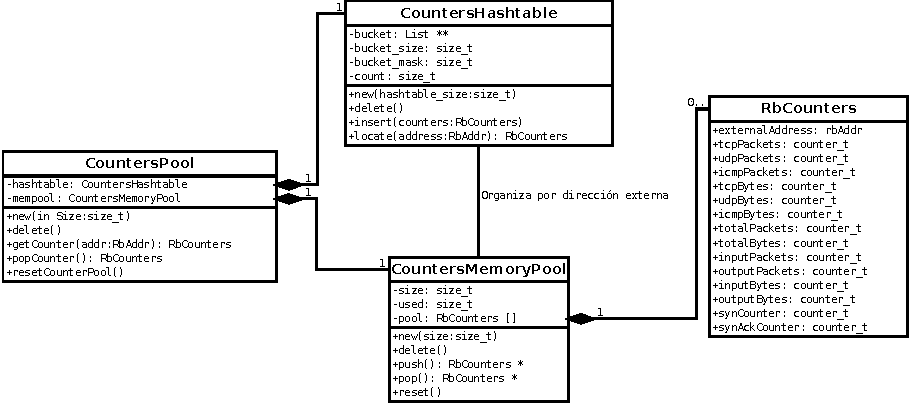
\includegraphics[width=\textwidth]{CapituloEstructura/Figuras/DiagramaClasesContadores-crop}
\caption{Diagrama de clases de la piscina de contadores}
\LABFIG{ClasesPoolContadores}
\end{figure}
%

A lo largo de la ejecución del programa, no se permitirá hacer nuevas reservas de memoria al \gls{SO} para 
nuevos contadores. En el caso de ataque, esto saturaría los recursos de los que dispone la máquina, por lo que tiene 
sentido ponerle un límite superior. Por otro lado, en caso de ataque repentino, no se debería perder tiempo en llamadas 
al \gls{SO} para pedir más memoria. Así pues, se dispondrá de un número limitado de contadores desde el inicio hasta el 
final de la ejecución del programa.

\subsubsection{Algoritmo del subcontador}
Tras ser enviado el paquete a una cola, le tocará ser procesado por un hilo contador. Cada hilo contador tiene 
asociadas dos piscinas de contadores\footnote{ver \SSSEC{Pool de contadores}.}. 

Cuando un nuevo paquete llega, la Función de Distribución\footnote{ver \SSEC{EstructuraCluster}.} lo habrá marcado como 
entrante o saliente, según la interfaz por la que ha entrado al Cluster. A partir de ahí, se extrae su \gls{IP} externa 
mediante el Algoritmo \ALG{ExtracciónIPExterna}.

\begin{algorithm}[htbp]
 \KwData{Paquete a analizar}
 \KwResult{Dirección del mismo }
 \eIf{paquete entrante}{
   ip externa $\gets$ ip origen\;
   }{
   ip externa $\gets$ ip destino\;
  }
 \caption{Algoritmo de extracción de IP externa}
 \LABALG{ExtracciónIPExterna}
\end{algorithm}

Tras ello, se pide a la piscina de contadores el contador asociado a la IP externa, y se actualiza la información 
pertinente, controlando siempre los errores como que la piscina esté llena y no pueda albergar ningún contador más.

En la \FIG{ActividadSubcontador} podemos ver el diagrama de actividad de esta función.

\begin{figure}[htbp]
\centering
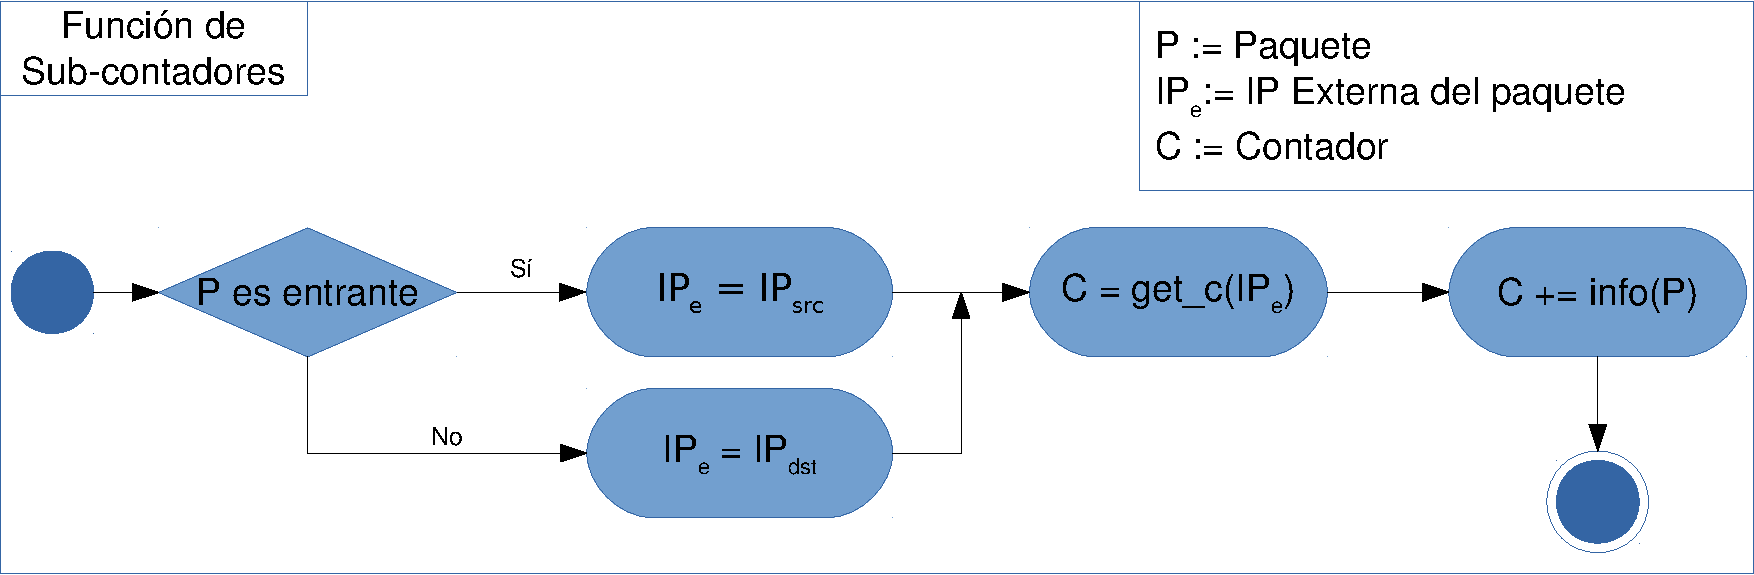
\includegraphics[width=\textwidth]{CapituloEstructura/Figuras/ActividadFuncionContador-crop}
\caption{Función de sub-contador}
\LABFIG{ActividadSubcontador}
\end{figure}
%

\subsection{Contador Maestro}\index{Contrador Maestro}
\subsubsection{Señal SIGALRM}\index{SIGALRM}
Para conseguir que la función del contador maestro se ejecute de una manera periódica, se usa la señal 
SIGALRM\index{Señales de GNU/Linux}\index{SIGALRM} de GNU/Linux (ver sección \SSEC{SIGALRM}). Cuando esta se produce, 
se activará una variable global \texttt{sigalrm\_received} y, si esta ya estaba activada en el momento que se produjo, 
se activará también \texttt{sigalrm\_accum}, como indicador de que \redborderddos{} no es capaz de procesar todo el 
flujo de tráfico.

\subsubsection{Mínima interrupción de los sub-contadores}
Los sub-contadores son la parte de \redborderddos que más carga de trabajo llevan. Es por eso por lo que se ha enfocado 
todo el diseño de la aplicación en hacerlos lo más escalable posible.

Sin embargo, es necesario recolectar los contadores y procesarlos en algún momento, con el fin de extraer los distintos 
estadísticos \gls{CUSUM}. Sería impensable bloquear los sub-contadores con el fin de extraer dichos estadísticos: Si la 
piscina está muy ocupada, la cola de paquetes se llenaría y nos veríamos obligados a tirar paquetes.

Para evitar detener los hilos sub-contadores un largo periodo de tiempo, se trabaja con punteros y con las variables 
cerrojo de la librería \gls{pthreads}\index{Librería pthread}. Cada hilo contador tiene reservados dos piscinas de 
contadores, y sólo usa en un periodo de tiempo una de ellas, que va llenando de contadores. Un puntero apunta al 
contador que está usando actualmente, situado en un vector que llamaremos \emph{Piscina Contadores}. Así, el contador 
que está usando el trabajador \emph{i} actualmente será \emph{Piscina contadores[i]}.

Cada hilo contador tiene asociado una variable cerrojo\index{Variable Cerrojo}, que bloquea cuando trabaja con su 
piscina. Cuando se activa la alarma del hilo principal, éste último bloquea dicha variable, e intercambia las piscinas 
de los hilos contadores, lo que se traduce en una simple asignación de punteros y esto, a su vez, se traduce como un 
tiempo mínimo de bloqueo.

Así pues, en el instante previo al lanzamiento de la alarma, el hilo contador ve una piscina llena de contadores, 
mientras que en el instante posterior ve una piscina nueva y limpia en la que almacenar. Para una descripción 
gráfica, ver \FIG{AntesSIGALRM} y \FIG{DespuesSIGALRM}.

\begin{figure}[htbp]
\centering
%\hfill
\subfloat[Instante antes de lanzar SIGALRM]%
   {\LABFIG{AntesSIGALRM}%
   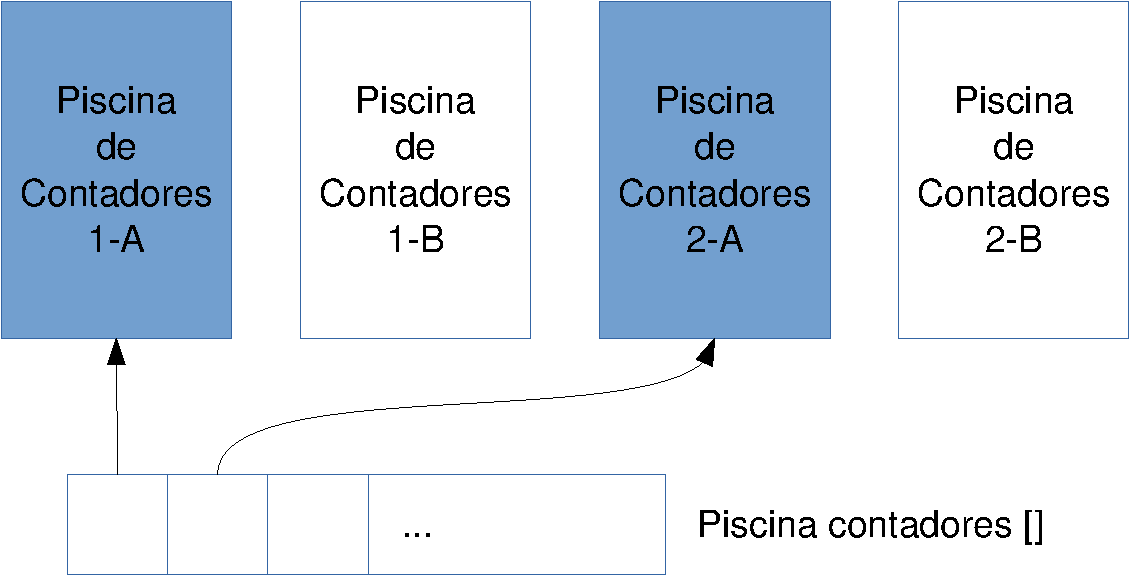
\includegraphics[width=0.45\textwidth]{CapituloEstructura/Figuras/DiagramaPoolsAntesSIGALRM-crop}}%
\hfill
\subfloat[Instante después de lanzar SIGALRM]%
 {\LABFIG{DespuesSIGALRM}%
 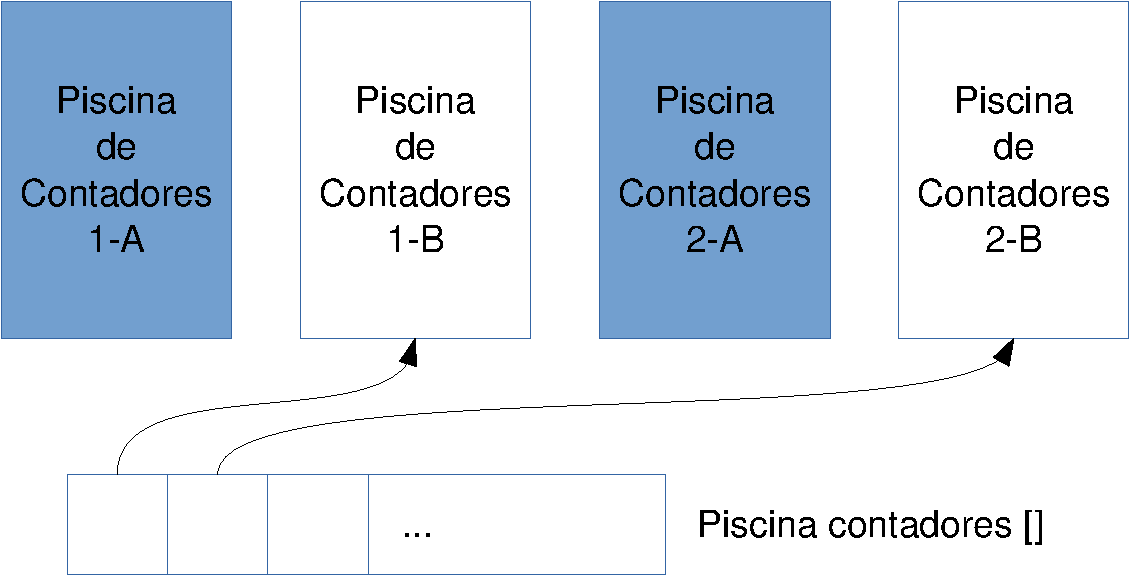
\includegraphics[width=0.45\textwidth]{CapituloEstructura/Figuras/DiagramaPoolsDespuesSIGALRM-crop}}%

\caption{Estado de las piscinas de contadores instantes antes y después de lanzar SIGALRM}
%\LABFIG{ActividadSubcontador}
\end{figure}
%

\subsubsection{Extración de estadísticos CUSUM}\LABSSSEC{ExtraccionEstadisticosCUSUM}

Tras intercambiar los contadores con el/los hilos contadores, el hilo maestro deberá extraer las estadísticas CUSUM de 
los mismos. Para ello, preparamos una estructura de datos con los parámetros de interés vistos en la 
\SSEC{Parametros de interés}. Por ello, de cada contador IP se debe extraer una muestra $x_i$ que indique el estado de 
las variables a controlar en ese momento.

Por comodidad, copiamos la estructura en \lstlistingname{} \ref{code:RbCusumStats}, y el algoritmo seguido para 
rellenarla en las ecuaciones desde \EQ{ExtractCusumTcpBytesRate} hasta \EQ{ExtractCusumInputOutputRate}.

\begin{align}
 \text{stats.tcp\_bytes\_percent}  &\gets \frac{\text{counters.tcp\_bytes   }}{\text{counters.total\_bytes}}
                                                                                    \LABEQ{ExtractCusumTcpBytesRate}\\
 \text{stats.udp\_bytes\_percent}  &\gets \frac{\text{counters.udp\_bytes   }}{\text{counters.total\_bytes}}\\
 \text{stats.icmp\_bytes\_percent} &\gets \frac{\text{counters.icmp\_bytes  }}{\text{counters.total\_bytes}}\\
%
 \text{stats.tcp\_pkts\_percent}   &\gets \frac{\text{counters.tcp\_pkts    }}{\text{counters.total\_pkts}}\\
 \text{stats.udp\_pkts\_percent}   &\gets \frac{\text{counters.udp\_pkts    }}{\text{counters.total\_pkts}}\\
 \text{stats.icmp\_pkts\_percent}  &\gets \frac{\text{counters.icmp\_pkts   }}{\text{counters.total\_pkts}}\\
%
 \text{stats.syn\_ack\_rate}       &\gets \frac{\text{counters.syn\_counter }}{\text{counters.ack\_counter}}\\
 \text{stats.input\_output\_prate} &\gets \frac{\text{counters.input\_pkts  }}{\text{counters.output\_pkts}}\\
 \text{stats.input\_output\_brate} &\gets \frac{\text{counters.input\_bytes }}{\text{counters.output\_bytes}}
                                                                                     \LABEQ{ExtractCusumInputOutputRate}
\end{align}

\begin{lstlisting}[language=C++,caption={Estructura estadísticos CUSUM}, breaklines=true, 
label=code:RbCusumStats,numbers=left,float=htbp]
typedef struct rb_cusum_stats_sample_s{
    double tcp_bytes_percent;   ///< TCP bytes/total bytes rate
    double udp_bytes_percent;   ///< UDP bytes/total bytes rate
    double icmp_bytes_percent;  ///< ICMP bytes/total bytes rate

    double tcp_pkts_percent;    ///< TCP paktes/total packets rate
    double udp_pkts_percent;    ///< UDP paktes/total packets rate
    double icmp_pkts_percent;   ///< ICMP paktes/total packets rate

    double syn_ack_rate;        ///< syn/ack rate

    double input_output_prate;   ///< Rate input/output packets
    double input_output_brate;   ///< Rate input/output bytes
}rb_cusum_stats_sample_t;
\end{lstlisting}

\subsubsection{Muestra completa de un estadístico CUSUM}
Como vimos en la \SEC{AlgoritmoCUSUM}, es necesario llevar el algoritmo CUSUM para el lado positivo y negativo ($C_i^+$ 
y $C_i^-$). Por tanto, con cada muestra debemos actualizar dos estadísticos \gls{CUSUM} por flujo o \gls{IP} externa.

Por ello, se debe crear una estructura que nos permita relacionar esas tres características. En cada ciclo del contador 
maestro, éste extraerá los contadores de los \texttt{CountersPool} vistos en \SSSEC{Pool de contadores} usando el 
método \texttt{popCounter} hasta que no haya más contadores (esto es, hasta que la misma devuelve \texttt{NULL}.

Por cada contador, extraemos una muestra $X_i$ como hemos visto en el \SSSEC{ExtraccionEstadisticosCUSUM}. Tras ello, 
aplicamos el algoritmo visto en la \SEC{AlgoritmoCUSUM}:

\begin{align}
 C_i^+ &= \max \left[0,\left\{C_{i-1}^+\left(x_i-\mu_0\right)\right\}-K\right] \LABEQ{CUSUMPositivo}\\
 C_i^- &= \max \left[0,\left\{C_{i-1}^-\left(x_i-\mu_0\right)\right\}-K\right] \LABEQ{CUSUMNegativo}
\end{align}

Donde $C_{i-1}$ es el contador almacenado en la anterior iteración.

No obstante, existe un problema con esta forma de actuar: es posible que en una iteración exista el $x_i$ de un 
contador, en la siguiente iteración no exista tráfico de esa dirección \gls{IP}, por lo que no se generaría ningún 
contador del mismo, y vuelva a existir el contador en la tercera iteración. De esa forma, si $T=-\mu_0-K$, $C_3$ 
quedaría:
\begin{align}
 C_3 = \max\left[0,C_1 + (x_3-T)\right] = \max\left[0,x_1-T+x_3-T\right] = 
       \max\left[0,x_1+x_3-2T\right] 
\end{align}
Sin embargo, al tener en cuenta $X_2=0$, $C_3$ debería quedar:
\begin{align}
 C_3 &= \max\left[0,C_1 + C_2 + (x_3-T)\right] = \max\left[0,x_1-T+0-T+x_3-T\right]
     =        \max\left[0,x_1 + x_3 -3T\right] 
\end{align}

Para salvar esa diferencia, tenemos dos opciones:
\begin{itemize}
 \item Escanear todo el espacio de direcciones CUSUM y actualizarlo.
 \item Almacenar, por cada CUSUM que se actualice, la marca de tiempo en la que fue actualizado.
\end{itemize}

Se elige, por razones de rendimiento, la segunda opción. Por tanto, la estructura para almacenar $C_i^+$ y $C_i^-$ 
quedan como se muestra en la \FIG{ClasesCusumSample}.

\begin{figure}[htbp]
\centering
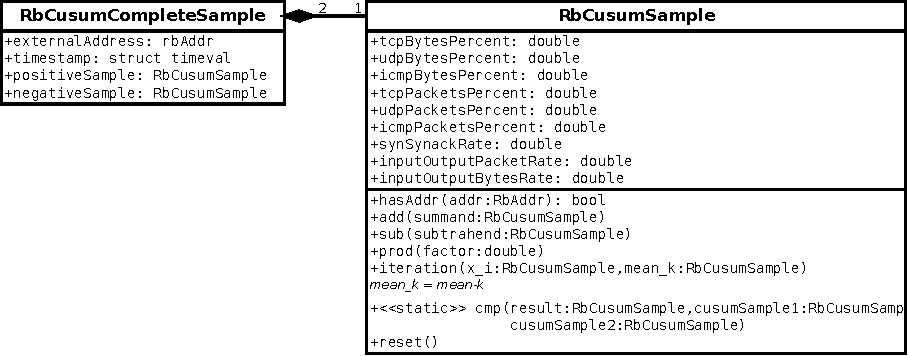
\includegraphics[width=\textwidth]{CapituloEstructura/Figuras/DiagramaClasesCusumSample-crop}
\caption{Diagrama de clases de las estructuras de almacenamiento de estadísticas CUSUM}
\LABFIG{ClasesCusumSample}
\end{figure}
%

Como funciones especiales que actúan sobre la estructura, se destacan \emph{iteration}, que realiza una iteración 
\gls{CUSUM} sobre la muestra, y \emph{cmp}, que guarda en una estructura del mismo tipo la comparación entre dos 
estructuras, aplicando el la comparación vista en Algoritmo\ALG{ComparacionFlotante} en cada miembro de la misma.

\subsubsection{Limpieza de estadísticos antiguos}\LABSSSEC{LimpiezaCusum}
Todo lo que se aprende, debe ser olvidado. Si pretendiésemos almacenar estadísticas \gls{CUSUM} por cada \gls{IP} que 
vemos indefinidamente, terminaríamos por saturar los contadores, y no podríamos seguir el comportamiento de ninguna 
dirección \gls{IP} más.

Por el momento, se reservará una cantidad fija de memoria para los estadísticos \gls{CUSUM}, y se almacenarán, a 
priori, en una lista de contadores \emph{libres}. A medida que se van necesitando, se almacenarán en otra lista de 
contadores \emph{en uso}. Es importante, desde el punto de vista del rendimiento, que la entrada de contadores en esta 
lista esté bien definida: O bien por la cabeza, o bien por la cola. A lo largo de este ejemplo, la entrada de 
estadísticos \gls{CUSUM} nuevos se realizará por la cabeza.

A intervalos de tiempo regulares, se realizará una limpieza de los contadores usados, comenzando por el lado inverso a 
la entrada de los mismos. En este ejemplo, el sentido elegido será la cola. Se elegirá un tiempo mínimo, a partir del 
cual, si el estadístico no ha sido actualizado tras esa marca de tiempo, será eliminado de la lista de 
estadísticos \emph{en uso} y pasará a la lista de \emph{libres}. Podemos ver este procedimiento en el 
Algoritmo\ALG{EliminacionContadoresAntigos} y en la \FIG{DiagramaActividadLimpiarLista}.

\begin{algorithm}
 \KwData{Lista de estadísticos cusum $l$, marca de tiempo $t$}
 \KwResult{Lista de estadísticos con sólo las entradas con marca de tiempo $t_0$ que cumplen $t_0>t$}
 \While{element $e \gets l.$last and $e.$timestamp $< t_0 $}{
	 usados.delete($e$)\;
	 libres.push($e$)\;
 }
 \caption{Procedimiento para la eliminación de contadores antiguos}
 \LABALG{EliminacionContadoresAntigos}
\end{algorithm}

\begin{figure}[htbp]
\centering
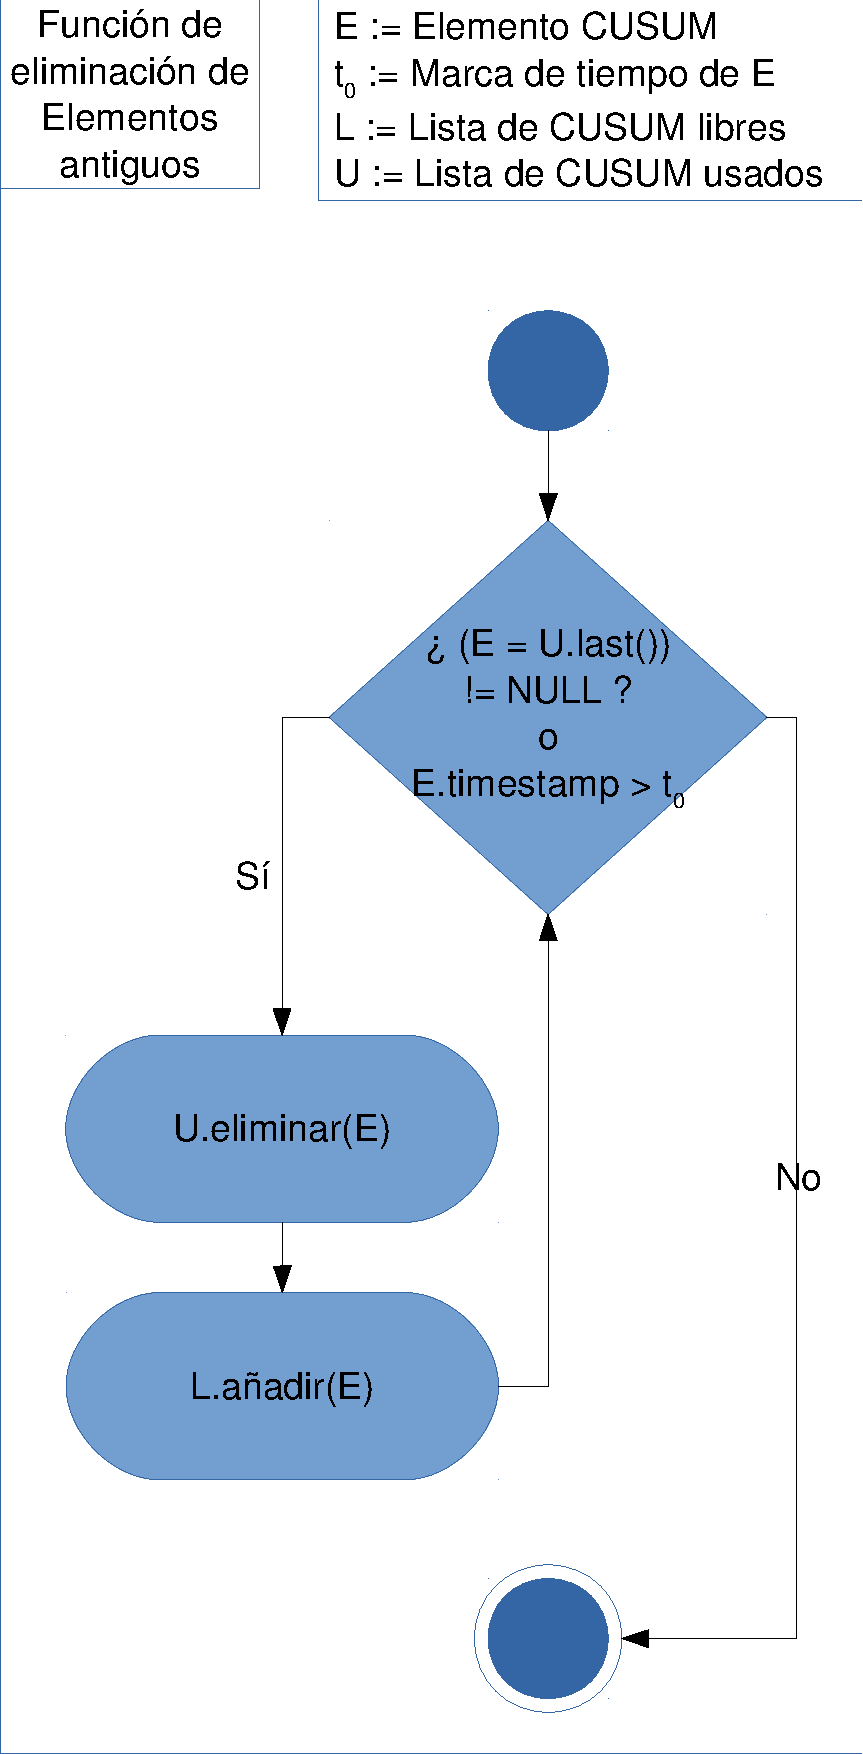
\includegraphics[width=0.4\textwidth]{CapituloEstructura/Figuras/ActividadFuncionLimpiarPoolCUSUM-crop}
\caption{Diagrama de actividad de la limpieza de estadísticos CUSUM antiguos}
\LABFIG{DiagramaActividadLimpiarLista}
\end{figure}
%

El orden de entrada y salida en la segunda lista no es relevante, si bien es preferible que esta actúe como una pila, 
con el fin de maximizar las probabilidades de que la memoria ocupada por los contadores se encuentre en la caché del 
procesador\footnote{Dicha caché eliminará las páginas que no han sido recientemente utilizadas. Si queremos volver a 
ellas, será necesario volver a recuperarlas de la RAM.}.

Cuando se use de nuevo un contador de la lista de contadores \emph{en uso}, esto es, se insertó en $C_i$ y se usó en 
$C_j j>i$, es necesario volver a colocarlo en la cabeza de la lista. Para ello, se deberá extraer de la misma, y volver 
a colocar en la cabeza. Si no se hiciese este paso, las marcas de tiempo de cada contador no estarían ordenadas en la 
lista, y la limpieza no sería efectiva.

Por ejemplo, si tenemos cinco flujos que están activos en un tiempo $t_i$, y nunca más vuelven a estar activos. Tras 
ellos, y sin haberse olvidado aún, llega un flujo en el instante $t_j j>i$ que, por ejemplo, se trata de un proceso 
automatizado que hace peticiones en un corto espacio de tiempo (por tanto, nunca olvidaremos ese flujo, ya que nunca 
será lo suficientemente antiguo).

Si no actualizamos la posición del elemento que ha llegado en $t_j$, y lo volvemos a colocar en la cabeza de la lista, 
nunca eliminaremos los elementos que llegaron antes.

\subsubsection{Pool de estadísticos CUSUM}

Al igual que ocurre con los contadores, el contador maestro necesita almacenar los diferentes estadísticos CUSUM que ha 
ido almacenando a lo largo del tiempo, y recuperarlos de una manera rápida. Para ello, se utiliza una estructura 
similar a la usada para almacenar y localizar los contadores: un Pool de estadísticos CUSUM.

Para ello, se utiliza una estructura similar a la vista en el \SSSEC{Pool de contadores}, pero necesita algunas 
diferencias. Mientras que la piscina de contadores tenía un ciclo de vida bien definido (nacía y moría en cada ciclo), 
esta estructura debe estar diseñada para vivir todo lo que viva el programa, por lo que necesita un método para 
eliminar entradas antiguas.

Por otro lado, no es necesario acceder, desde fuera de la misma, a los nodos almacenados de una manera 
lineal, es decir, como una lista.

\begin{figure}[htbp]
\centering
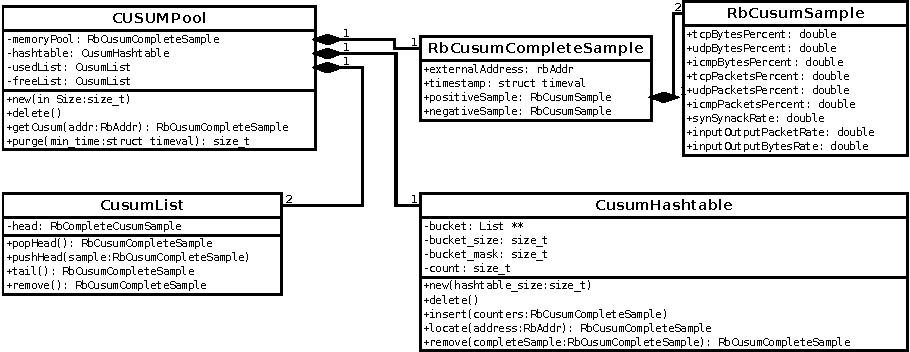
\includegraphics[width=\textwidth]{CapituloEstructura/Figuras/DiagramaClasesCUSUM-crop}
\caption{Diagrama de clases de la piscina de estadísticas CUSUM}
\LABFIG{ClasesCusumPool}
\end{figure}
%

Así pues, el diagrama de clases de la piscina de estadísticos \gls{CUSUM} se ve reflejado en \FIG{ClasesCusumPool}. 
Además del constructor y destructor, las funciones a destacar son \emph{getCusum}, que obtendrá la muestra completa 
\gls{CUSUM} que le indiquemos, y \emph{purge}, que eliminará de la piscina los contadores antiguos, siguiendo el 
algoritmo del \SSSEC{LimpiezaCusum}. Debido a ello, existen en la estructura las listas de estadísticos \emph{freeList} 
y \emph{usedList}.

En dichas listas podemos:
\begin{itemize}
 \item Añadir un elemento por la cabeza (inserción de un estadístico CUSUM).
 \item Eliminar un elemento por la cabeza (para extraer un elemento de la lista de libres).
 \item Acceder al elemento de la cola (para hacer la purga).
 \item Eliminar un elemento aleatorio de la lista.
\end{itemize}

Por último, para accesos aleatorios a los elementos tenemos la Tabla HASH, al igual que ocurría con la piscina de 
contadores. Es importante destacar que, al purgar los elementos, además de eliminarlos de la lista de elementos usados 
es necesario eliminarlos también de la tabla HASH. De otra forma, tendremos la entrada a un elemento eliminado.

\subsubsection{Algoritmo del contador maestro}

Con los conceptos vistos bajo esta sección, el algoritmo del contador maestro queda como se muestra en Algoritmo 
\ALG{AlgoritmoContadorMaestro} y en \FIG{ActividadContadorMaestro}\footnote{En la figura se han eliminado los 
condicionales de estado \texttt{APRENDIZAJE}, ya que es fácil de extrapolar y hacía innecesariamente grande la figura}. 
En ellos, se usa la función \texttt{alarma\_ddos}, la cual se describirá posteriormente en la \SSEC{Decisor}.

Falta añadir que, destinado a extraer la media y desviación típica del tráfico, el contador dispone de un vector de 
estadísticos \gls{CUSUM} de longitud suficiente para almacenar una muestra \gls{CUSUM} por cada iteración que tendrá en 
el periodo de aprendizaje. Cuando dicho vector está lleno, el sistema extrae la media y la desviación típica con la que 
trabajará el resto del tiempo.

Para facilitar la lectura del algoritmo, se recomienda hacerlo en cinco pasadas:

\begin{description}
 \item [Periodo de aprendizaje] Suponiendo que estamos en periodo de aprendizaje, que abarcarían el algoritmo desde la 
línea \ref{algoline:inicioAprendizaje} hasta \ref{algoline:finAprendizaje}
 \item [Periodo de defensa sin alertas] A continuación, se leería una iteración del periodo de defensa sin alertas, que 
sería leer todo el algoritmo sin entrar en los bloques condicionales que producen una llamada a la función 
\texttt{alarma\_ddos}, esto es, las líneas \ref{algoline:inicio1Defensa}-\ref{algoline:fin1Defensa} y 
\ref{algoline:2DefensaNoAlerta}. Tras ello, se volvería al estado de defensa.
 \item[Periodo de defensa con alertas] Camino seguido si, durante el periodo de defensa recibimos una alerta, esto es, 
un contador $C_i$ sobrepasa el umbral. Esto es, líneas \ref{algoline:inicio1Defensa}-\ref{algoline:fin1Defensa} y 
\ref{algoline:InicioDefensaAlerta}-\ref{algoline:FinDefensaAlerta}. Tras ello, pasamos al estado de alerta.
 \item[Estado de alerta] Si durante una iteración se lanza alguna alarma, estaremos a partir de esa 
iteración y en la siguiente en estado de alarma. Así, la siguiente iteración cubrirá las líneas 
\ref{algoline:inicioAlerta}-\ref{algoline:finAlerta1}, y marcará las direcciones IP nuevas como atacantes en el bloque 
condicional de la línea \ref{algoline:condAlerta}. Si, durante este estado, no se entra en la condición anterior, ni 
ningún contador supera el límite, se volverá al estado de defensa. En caso contrario, el sistema permanecerá en alerta.
\end{description}

\LinesNumbered
\begin{algorithm}
	\KwData{Piscina de contadores $P_C$, piscina de estadísticos \gls{CUSUM} $P_E$}
	\KwResult{Actualización de la piscina de contadores}
	alertas = falso\;
	\While{listaContadores no vacía}{
		Contador $C$ = extraer cabeza de $P_C$ \label{algoline:inicioAprendizaje}\label{algoline:inicio1Defensa}
		                                       \label{algoline:inicioAlerta}\;
		Estadísticos CUSUM $X$ = extraídos de contador $C$\;
		IPAddr $E_{IP}$ = Dirección \gls{IP} externa de $C$\;
		Stats $S_{IP}$ = CUSUM con clave $E_{IP}$ en $P_E$  \label{algoline:fin1Defensa}\label{algoline:finAlerta1}\;
		\eIf{Periodo de aprendizaje}{
			Añadir $X$ al vector de aprendizaje $V_A$\;
			\If{$V_A$ lleno}{
				\tcp{Fin del periodo de aprendizaje}
				Almacenar media $\mu_0$ y desviación típica $\sigma$
				Estado = \texttt{DEFENSA}
			} 
		}{                                                              \label{algoline:finAprendizaje}
			\If{$S_{IP}$ es nuevo y estamos en alerta}{                   \label{algoline:condAlerta}
				alarma\_ddos($C_{i}$)                                       \label{algoline:AlarmaNuevaIp}\;
				estado alerta\;
				alertas = verdadero\;
			}
			Iteración \gls{CUSUM} con $C_{i-i}=S_{IP},x_i=X$, usando $\mu_0$ y $\sigma$ Guardar en $S_{IP}$
                                                \label{algoline:2DefensaNoAlerta}\label{algoline:InicioDefensaAlerta}\;
			\If{$C_{i-1} > \text{Límites }H$}{
				alarma\_ddos($C_{i}$)                   \label{algoline:AlarmaUmbralSuperado}\;
				Estado = \texttt{ALARMA}\;
				alertas = verdadero\;
			}                                         \label{algoline:FinDefensaAlerta}
		}
	}
	\If{alertas = verdadero}{
		Estado = \texttt{DEFENSA}\;
	}
\caption{Algoritmo usado en el contador maestro}
\LABALG{AlgoritmoContadorMaestro}
\end{algorithm}
\LinesNotNumbered


\begin{figure}[htbp]
\centering
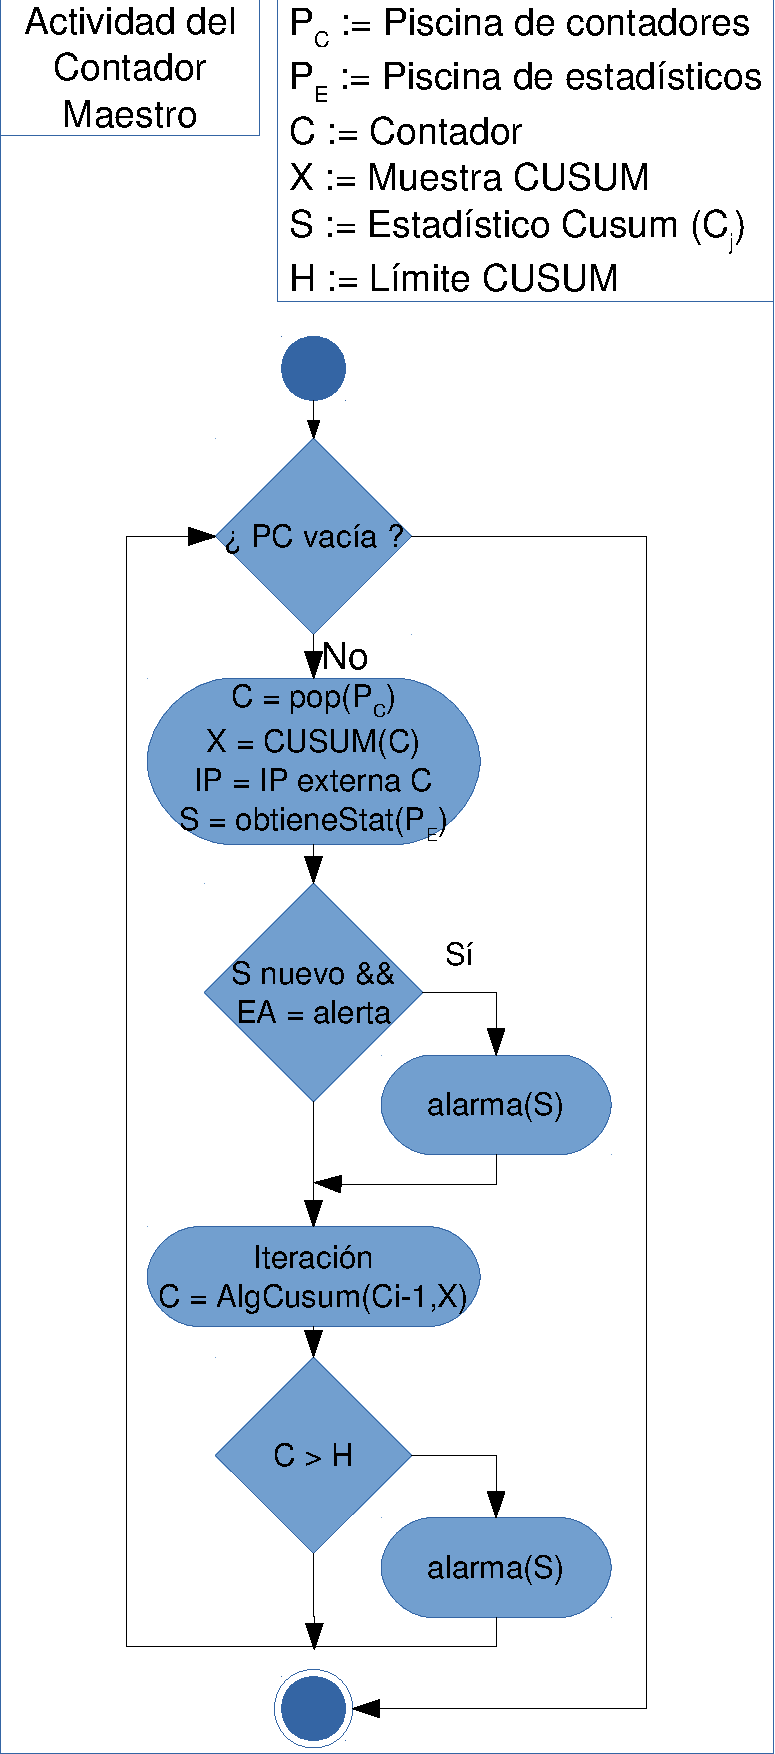
\includegraphics[height=0.5\textheight]{CapituloEstructura/Figuras/ActividadContadorMaestro-crop}
\caption{Diagrama de Actividad del Contador Maestro}
\LABFIG{ActividadContadorMaestro}
\end{figure}
%

\subsection{Decisor}\index{Decisor}\LABSSEC{Decisor}
Como último paso, resta decidir qué IP es maliciosa y qué IP no lo es, mediante el algoritmo \gls{CUSUM} 
(Ecuaciones \EQ{CUSUMPositivo} y \EQ{CUSUMNegativo}). Una vez calculado $C_i$ siguiendo Algoritmo 
\ALG{AlgoritmoContadorMaestro}, se comparará con un valor $Threshold$, que se tendrá pre-cacheado para mayor comodidad.

Tras ello, se examinará la comparación, y se emitirá un mensaje de alerta\index{Alerta}. Como ya hemos dicho, la 
alerta será emitida por el protocolo Kafka en formato \gls{json}.

\begin{lstlisting}[language=json,caption={Ejemplo de alarma por umbral superado}, breaklines=true, 
label=code:ejemplosAlarmaUmbral,numbers=left,float=htbp]
{
	"timestamp": 1410602387, 
	"extern_ip": "8.8.8.8", 
	"positive_tcp_bytes_percent_value": 25.000000,
	"negative_udp_bytes_percent_value": 6.666667, 
	"positive_udp_pkts_percent_value": 13.333333, 
	"reason": "threshold"
}
\end{lstlisting}

\begin{lstlisting}[language=json,caption={Ejemplo de alarma por nueva IP}, breaklines=true, 
label=code:ejemplosAlarmaNuevaIP,numbers=left,float=htbp]
{"timestamp":1410622605,"extern_ip":"8.8.8.8","reason":"New IP in alarm time"}
\end{lstlisting}


En \lstlistingname{} \ref{code:ejemplosAlarmaUmbral} vemos el ejemplo de la alarma emitida si se supera el umbral 
\gls{CUSUM}. Esto es, la alarma que se emite en la línea \ref{algoline:AlarmaUmbralSuperado} del algoritmo 
\ALG{AlgoritmoContadorMaestro}.

En el mensaje \gls{json} podemos ver los campos \texttt{timestamp}, que indican el momento 
de la alerta en formato UNIX time\index{Unix time}\footnote{Número de segundos transcurridos desde el 1 de enero de 1970 
a las 00:00}, la dirección que ocasionó la alerma, y los distintos campos que han superado el umbral positivo o 
negativo. Las unidades de estos están en ``desviaciones típicas'', esto es, un valor de $25$ indica que $C_i$ estaba, en 
ese momento, a $25\sigma$.

Por último, se indica que la razón del mensaje ha sido superar el valor límite. Si lo comparamos con el mensaje de 
\lstlistingname{} \ref{code:ejemplosAlarmaNuevaIP}, vemos que no aparecen ninguno de los campos relacionados con la 
superación del valor límite y, en su lugar, sólo aparece que la alarma está causada por ser una \gls{IP} no vista 
previamente en periodo de alerta. Este mensaje sería el enviado en la línea \ref{algoline:AlarmaNuevaIp} del Algoritmo
\ALG{AlgoritmoContadorMaestro}.

\section{Conclusiones}
\redborderddos{} es capaz de analizar el tráfico, aplicando técnicas eficientes de almacenamiento de datos y uso de la 
memoria y miltiprocesamiento, tales como las tablas hash, el alineamiento de los datos en memoria y el uso del 
miltihilo, respectivamente. Su diseño modular permite que cada procesador dedique su tiempo a realizar una única tarea, 
de una forma exclusiva, y se usan técnicas rápidas de IPC tales como el intercambio de piscinas que, si bien usan mucha 
memoria, son necesarias si queremos conseguir el rendimiento esperado.

Externamente, \redborderddos{} necesita como mínimo dos interfaces de entrada de datos, que serán una copia del tráfico 
saliente y entrante a los activos a proteger. Podemos, a partir de ahí, usar tantas interfaces como queramos, tanto de 
entrada como de salida.

Internamente, un clúster redirigirá el tráfico hacia varios hilos contadores, según el flujo de datos al que 
pertenezcan. Ellos almacenarán las características del tráfico, y contaran paquetes u octetos de distintas 
características según el protocolo al que pertenezcan, que sean salientes o entrantes, y, si es \gls{TCP}, que tengan 
determinadas banderas activadas.

Tras ello, un contador maestro aplicará el algoritmo \gls{CUSUM} a los contadores, para finalmente decidir si el flujo 
es legítimo o, por el contrario, se trata de un flujo atacante.

\section{Resúmenes}%%%%%%%%%%%%%%%%%%%%%%%%%%%%%%%%%%%%%%%
\begin{Resumen}[Alcance de \redborderddos]
\redborderddos{} intenta detectar los ataques de \gls{DDoS} por inundación, quedando fuera del alcance del proyecto los 
ataques semánticos.
\end{Resumen}

\begin{Resumen}[Nociones previas: El lenguaje de programación C]
\subsection*{Números en coma flotante}
\begin{flalign*}
  &\begin{cases}
    \text{Se intenta representar con $N$ estados un conjunto $\infty \rightarrow$ imprecisión} \\
    \text{Puede ocurrir que }(a \cdot b) \cdot c \neq a \cdot (b \cdot c) \\
    \text{Se hace necesario comparar con épsilon: $\left|a - b\right| < \epsilon \rightarrow a = b$}
  \end{cases}&
\end{flalign*}\\

\subsection*{Estructuras de datos básicas}
\begin{flalign*}
  &\begin{cases}
    \text{Vector}
    \begin{cases}
      \text{Posiciones contiguas de memoria} \\
      \text{Fácil acceso aleatorio. Dificil inserción de elementos}
    \end{cases}\\
    \text{Lista enlazada}
    \begin{cases}
      \text{Nodos diseminados por la memoria}\\
      \text{Cada elemento apunta al siguiente}\\
      \text{Variaciones: Doblemente enlazadas, etc}
    \end{cases}\\
    \text{Pilas}
    \begin{cases}
      \text{Contenedor que sólo se puede insertar y extraer en un sentido} \\
      \text{Se puede implementar con vector y con lista enlazada}
    \end{cases}\\
    \text{Tabla HASH}
    \begin{cases}
      \text{Vector de listas enlazadas} \\
      \text{Cada elemento tiene una clave} \\
      \text{La clave marca la posición del elemento} \\
      \text{Aplicar HASH ayuda a repartir elementos} \\
      \quad\text{Acceso aleatorio vector más rápido que lista enlazada} \\
      \text{Acceso aleatorio rápido} \\
      \text{Inserción/eliminación rápida}
    \end{cases}
  \end{cases}&
\end{flalign*}\\

\subsection*{Programación multihilo}
\begin{flalign*}
  &\begin{cases}
    \text{Hilo o proceso ligero: Unidad de ejecución independiente} \\
    \text{Modificación de memoria concurrente $\rightarrow$ Resultado indeterminado} \\
    \text{Región crítica}\\
    \quad\text{Zona de memoria que puede ser modificada por dos hilos}\\
    \text{Variables cerrojo}\\
    \quad\text{Protegen regiones críticas}
  \end{cases}&
\end{flalign*}\\

\subsection*{Alineación de memoria}
\begin{flalign*}
  &\begin{cases}
    \text{Si la memoria no está alineada, se requieren más instrucciones} \\
    \text{Memoria no alineada $\rightarrow$ Pérdidas de rendimiento}\\
    \text{Región crítica}\\
    \quad\text{Zona de memoria que puede ser modificada por dos hilos}\\
    \text{Variables cerrojo}\\
    \quad\text{Protegen regiones críticas}
  \end{cases}&
\end{flalign*}\\
 
\subsection*{Señales en LINUX}
\begin{flalign*}
  &\begin{cases}
    \text{Mecanismo de comunicación inter-proceso (IPC)}\\
    \text{Manejador de señal}\\
    \quad\text{Si el proceso recibe una señal $S_0$, se llama al manejador}\\
    \quad\text{Aleatoriedad en el momento de recibir la señal $\rightarrow$ concurrencia}\\
    \text{\texttt{SIGALRM}: Se programa recibir una señal $S_0$ en un tiempo $t_0$}\\
    \text{Se puede usar, con precaución, para eventos periódicos}
  \end{cases}&
\end{flalign*}\\

\end{Resumen}

\begin{Resumen}[Vista externa]
\begin{flalign*}
  &\begin{cases}
    \text{Situación física}
    \begin{cases}
      \text{Un puerto SPAN clona los paquetes hacia \redborderddos}\\
      \text{Se debe distinguir entre entrantes y salientes por puerto}\\
      \text{Si se quiere detener, un elemento externo debe bloquear}
    \end{cases} \\
%
	  \text{Envío del ataque mediante Kafka}
  \end{cases}&
\end{flalign*}
\end{Resumen}

\begin{Resumen}[Estructura interna]
\subsection*{Clúster}
\begin{flalign*}
 &\begin{cases}
   \text{Capaz de repartir paquetes entre hilos según origen-destino $\left(s_{ip},d_{ip}\right)\rightarrow n$}\\
   \text{Simétrico: $\left(ip_0,ip_1\right)\rightarrow n \Rightarrow \left(ip_1,ip_0\right) \rightarrow n$}\\
   \text{Podemos decir que reparte flujos}
 \end{cases}&
\end{flalign*}

\subsection*{Sub-contador}
\begin{flalign*}
 &\begin{cases}
   \text{Cuenta características de los flujos: tamaño, protocolo, etc.}\\
   \text{Usa una tabla hash para almacenar y recuperar los contadores por flujo}\\
   \text{Identifica flujos por \gls{IP} externa}
 \end{cases}&
\end{flalign*}

\subsection*{Contador maestro}
\begin{flalign*}
  &\begin{cases}
    \text{Sincronizado con \texttt{SIGALRM}}\\
    \text{Recoge los contadores de los hilos sub-contadores.}\\
    \text{Mínima interrupción: Intercambio de pools $\rightarrow$ punteros}\\
    \text{Extrae, por contador recogido, los parámetros \gls{CUSUM}}\\
    \text{Aplica el algoritmo \gls{CUSUM} con su muestra anterior por flujo}\\
    \text{Necesita eliminar las muestras antiguas para no agotar la memoria}
  \end{cases}&
\end{flalign*}

\subsection*{Decisor}
\begin{flalign*}
  &\begin{cases}
    \text{Intercalado en el contador maestro}\\
    \quad\text{1 iteración CM $\rightarrow$ 1 iteración decisor.}\\
    \text{Envía alarma indicando el tipo (umbral / nueva IP en alarma}\\
    \quad\text{Si alarma por límites $\rightarrow$ qué límites y cuánto}\\
  \end{cases}&
\end{flalign*}
\end{Resumen}

